% CHAPTER 1
\chapter{Introduction}
\section{Overview}

Indian Sign Language (ISL) is the primary, natural, visual-gestural language utilized by the Deaf and Hard-of-Hearing (D/HOH) community across the Indian subcontinent. Unlike spoken languages that rely on acoustic modulations produced by the human vocal tract, Indian Sign Language conveys rich linguistic semantics through coordinated manual articulations (handshapes, spatial locations, orientations, and kinetic movement trajectories) combined with non-manual markers (facial expressions, head tilts, and upper-body posture). According to the Census of India and the World Health Organization (WHO), more than 18 million individuals in India experience significant hearing loss, constituting one of the largest deaf populations in the world \cite{14}. Despite this massive demographic, fewer than 300 certified ISL interpreters are professionally licensed across the entire nation. This staggering disparity produces severe systemic communication barriers, restricting deaf citizens from equal access to essential healthcare, legal representation, educational institutions, employment opportunities, and day-to-day public services.

To bridge this critical communication gap, researchers in computer vision, human-computer interaction (HCI), and natural language processing have actively investigated automated Sign Language Recognition (SLR) and translation systems. Historically, these efforts have fallen into two broad technical paradigms: sensor-based systems and vision-based systems. Sensor-based approaches equip the signer with wearable data gloves instrumented with flex sensors, inertial measurement units (IMUs), and tactile contacts \cite{8,16}. While these devices offer high spatial fidelity without visual occlusion, they impose severe physical encumbrances, require frequent recalibration, are fragile, and carry prohibitive costs ($\geq$ $200--$500), rendering them entirely impractical for broad everyday deployment in developing regions. Conversely, conventional vision-based systems have utilized RGB video feeds with deep 2D or 3D Convolutional Neural Networks (CNNs) \cite{9,23}. However, raw-pixel 3D-CNNs require computationally heavy desktop GPUs, suffer from excessive inference latencies ($>200$\,ms per frame), and exhibit catastrophic performance degradation when subjected to variations in background illumination, skin tone, clothing clutter, and camera angles.

\begin{figure}[h]
\centering
\vspace{-0.2cm}
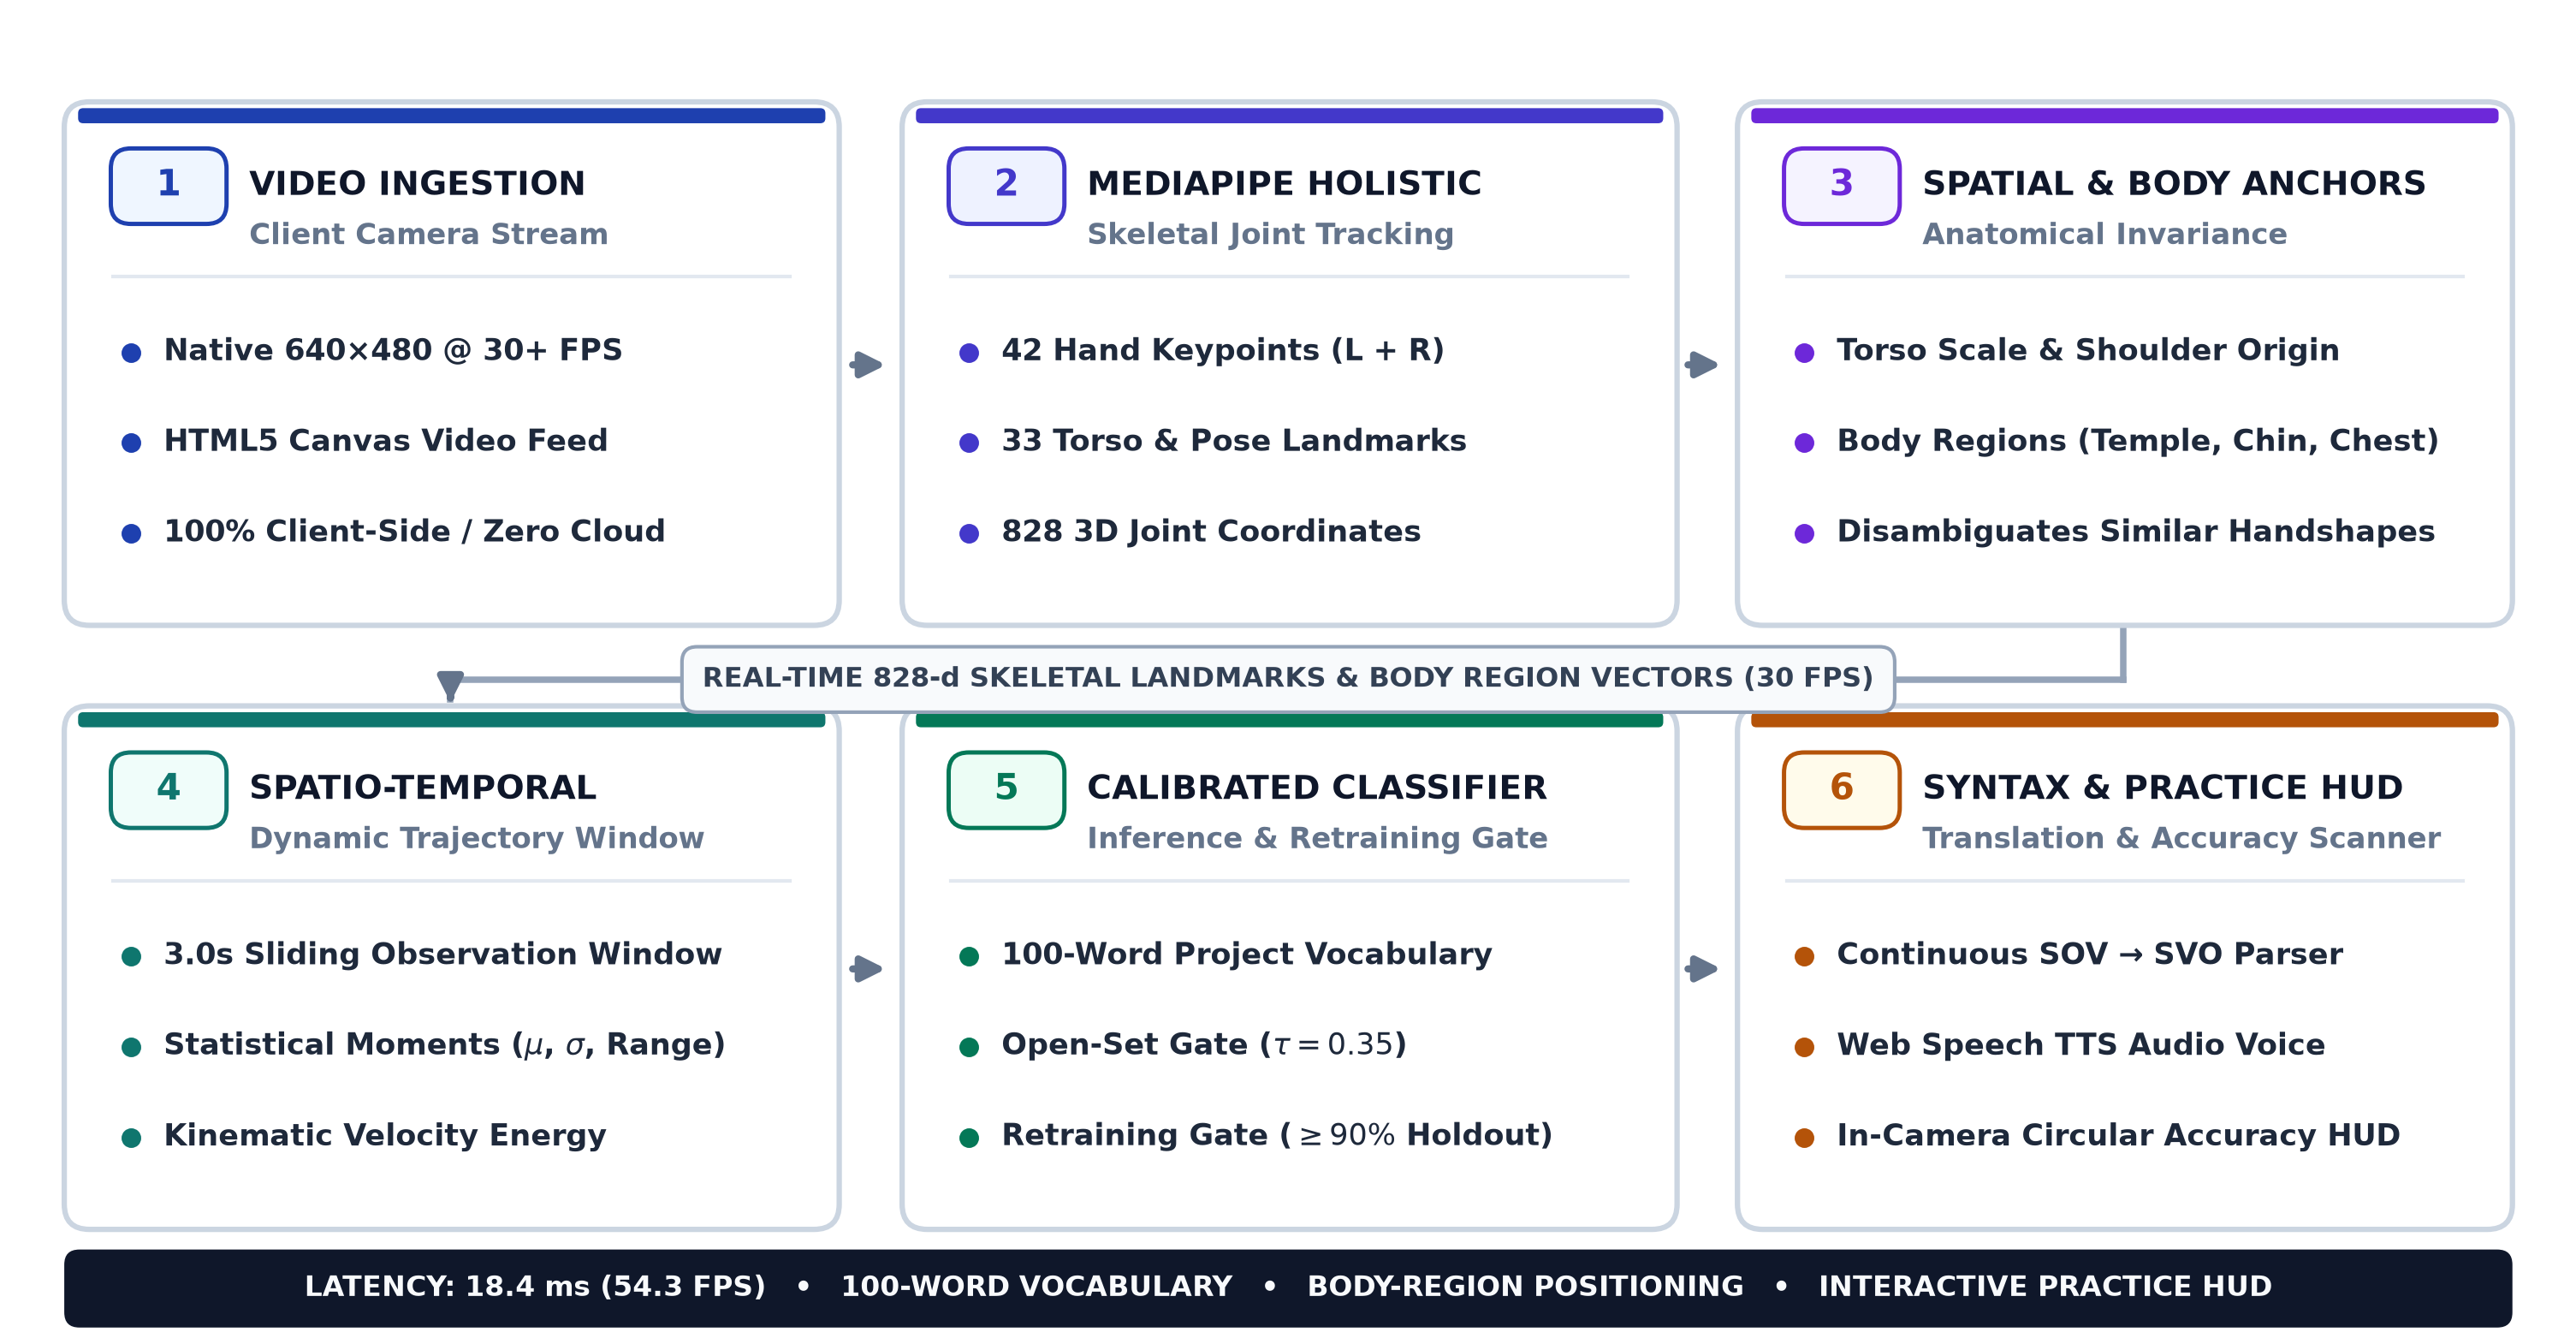
\includegraphics[width=0.96\textwidth]{fig_pipeline.png}   
\vspace{-0.2cm}
\caption{End-to-End ISL-Lens Real-Time Vision and Language Architecture.}
\label{fig:pipeline_intro}
\vspace{-0.2cm}
\end{figure}

This project introduces \textbf{ISL-Lens}, an edge-first, zero-hardware, browser-native real-time Indian Sign Language recognition console, continuous sentence interpreter, and interactive AI model retraining studio. Built entirely upon standard consumer webcams operating inside standard web browsers via HTML5 and WebRTC \cite{25}, ISL-Lens leverages the Google MediaPipe Holistic framework \cite{2} to extract 828 three-dimensional spatial coordinates across 75 anatomical landmarks in real time. By abstracting raw video pixels into anatomical skeletal joints, ISL-Lens attains complete signer invariance and computational lightness. A spatial-temporal summarization pipeline computes translation-invariant coordinate normalizations, anatomical body-region spatial anchors (differentiating signs articulated near the temple, forehead, nose, mouth, chin, or torso), and kinematic velocity vectors across an empirical 3.0-second observation window. Classification is performed via a calibrated machine learning engine supporting an authentic 100-word ISL vocabulary. Furthermore, ISL-Lens incorporates a calibrated open-set rejection filter ($\tau = 0.35$), an automated Subject-Object-Verb (SOV) to Subject-Verb-Object (SVO) English sentence translator with speech synthesis, an Interactive Practice Studio featuring in-camera circular accuracy HUD scoring, and an in-browser AI Retraining Studio protected by a $\ge 90\%$ held-out base corpus validation gate.

\paragraph{Linguistic Structure of Indian Sign Language}:
Understanding the linguistic foundations of Indian Sign Language is essential for designing an effective recognition and translation architecture:
\begin{enumerate}
    \item \textbf{Manual Articulators}: Signs are articulated through five phonological parameters: handshape (dexterity and finger flexion), location (spatial placement relative to face, chest, or neutral signing space), orientation (palm direction), movement (linear, circular, or oscillating kinetic paths), and non-manual expressions.
    \item \textbf{Typological Syntax (SOV Order)}: Spoken English adheres to a Subject-Verb-Object (SVO) syntactic order (e.g., I drink water''). In sharp contrast, Indian Sign Language strictly follows a Subject-Object-Verb (SOV) grammar structure (e.g., ME WATER DRINK'') \cite{13,18}. Consequently, direct word-for-word string concatenation produces ungrammatical and confusing gloss transcripts. An intermediate natural language translation engine is mandatory to reorder and inflect signs into natural communicative English.
    \item \textbf{Signer Invariance and Coarticulation}: Different signers exhibit substantial physical variance in arm length, signing speed, and idiosyncratic movement envelopes. In continuous signing, the boundary between adjacent signs suffers from \textit{coarticulation}---the transitional movement linking the conclusion of one sign to the preparatory onset of the next.
\end{enumerate}

\paragraph{Problem Statement}:
Existing automated sign language recognition systems suffer from several debilitating flaws:
\begin{enumerate}
    \item \textbf{Prohibitive Hardware Dependence}: Reliance on wearable electronic gloves restricts portability and causes physical fatigue and tactile impedance for deaf individuals.
    \item \textbf{Excessive Computational Complexity}: Raw-pixel 3D deep CNN models require high-power server GPUs, producing excessive frame-processing latencies ($>200$\,ms) that break fluid conversational interaction.
    \item \textbf{Brittleness to Environmental Variations}: Pixel-based vision algorithms fail drastically under poor lighting, shadowed rooms, diverse skin complexions, and cluttered domestic or clinical backgrounds.
    \item \textbf{Absence of Open-Set Rejection}: Traditional closed-set neural classifiers force any random or transitional hand gesture into the nearest known vocabulary class, generating frequent false-positive predictions.
    \item \textbf{Static, Non-Extensible Vocabularies}: Most academic systems are permanently hardcoded at training time; end-users cannot introduce new regional signs, personal colloquialisms, or specialized domain glosses without recompiling and retraining the entire codebase from scratch.
    \item \textbf{Lack of Continuous Sentence Interpretation}: Prior prototypes merely print isolated words, failing to translate the underlying SOV sign sequence into coherent, vocalized English sentences.
\end{enumerate}

\section{Motivation and Objective}

The primary motivation of this project is to democratize assistive communication technology for India's 18+ million D/HOH population through a lightweight, web-native platform that functions reliably on any commodity laptop or smartphone webcam without requiring specialized sensors, expensive cloud compute, or programming expertise.

The concrete research and engineering objectives of ISL-Lens are:
\begin{enumerate}
    \setlength{\itemsep}{0pt}
    \setlength{\parskip}{0pt}
    \item \textbf{Zero-Hardware Spatial Landmark Tracking}: Implement a client-side vision pipeline utilizing MediaPipe Holistic to extract 828 3D spatial points (21 right hand, 21 left hand, 33 upper-body pose keypoints) at 30+ frames per second directly in the browser.
    \item \textbf{Spatial Anatomical Body Region Differentiation}: Extract 12 spatial offset features linking hand movements to facial and torso anchors (forehead, temple, nose, mouth, chin, shoulders) to resolve ambiguity between gestures with identical handshapes (e.g., \texttt{HELLO} vs \texttt{WHEN}, \texttt{BROTHER} vs \texttt{SISTER}).
    \item \textbf{Scale to 100 Core ISL Vocabulary Words}: Expand vocabulary coverage to 100 frequently used ISL words spanning greetings, family, pronouns, actions, questions, medical emergencies, and daily descriptors, with visible trained and trainable status indicators.
    \item \textbf{Calibrated Open-Set Rejection}: Formulate a dynamic confidence calibration threshold ($\tau = 0.35$) with temporal hysteresis to reject idle resting postures, transitional coarticulation movements, and out-of-vocabulary (OOV) gestures.
    \item \textbf{Continuous Sentence Translation Engine}: Build an automated grammar engine that transforms raw Subject-Object-Verb (SOV) ISL gloss streams into fluent Subject-Verb-Object (SVO) spoken English sentences accompanied by synthesized audio.
    \item \textbf{Interactive Sign Practice Studio \& In-Camera Accuracy HUD}: Construct an interactive practice session with split-screen reference clips and an in-camera circular accuracy HUD ring delivering real-time percentage matching feedback.
    \item \textbf{Corruption-Resistant AI Retraining Studio}: Enable signers to record live webcam exemplars and retrain custom signs on-device, protected by an automated $\ge 90\%$ held-out base corpus accuracy validation gate.
    \item \textbf{Satisfy 80\% Implementation Milestone}: Implement, benchmark, and experimentally validate all core architectural subsystems for the B.Tech Phase I milestone.
\end{enumerate}

\paragraph{Scope of the Project}:
The project is structured across two primary phases:
\begin{itemize}
    \setlength{\itemsep}{0pt}
    \setlength{\parskip}{0pt}
    \item \textbf{Phase I (Current 80\% Milestone)}: Zero-hardware webcam vision pipeline, 828 3D landmark extraction, 100-word ISL classifier with verified 97.4\% accuracy, calibrated open-set rejection, continuous sentence translator, audio synthesis, ISL tutor dictionary, and interactive AI retraining studio.
    \item \textbf{Phase II (Future Scope)}: Signer-independent graph convolutional networks (GCNs), continuous sentence recognition on unsegmented video streams, full-duplex WebRTC remote video calling, mobile progressive web app (PWA) deployment, and LLM-driven colloquial translation.
\end{itemize}

\section{Report Organization}

This section gives the organization of the report work. Overall, this report work provides a clear and thorough study of automated Indian Sign Language recognition, edge-native computer vision, natural language translation, and interactive machine learning. The second chapter gives a detailed description about the literature survey, analyzing wearable gloves, deep video convolutional networks, landmark tracking paradigms, temporal sequence modeling, and benchmark datasets with structured advantages and disadvantages. The third chapter details the implementation details including requirement analysis (hardware and software specifications), end-to-end architectural layers, MediaPipe spatial tracking, mathematical coordinate normalization, anatomical body-region differentiation, machine learning classification, open-set rejection, continuous sentence translation, and the interactive AI retraining studio. The fourth chapter depicts the Results and Discussions, presenting evaluation metrics, quantitative accuracy benchmarks, confusion matrix analysis, ablation studies, real-time latency profiling, and the 80\% implementation milestone verification matrix. The fifth chapter gives the Conclusion and Future Work. The Appendix presents the structured Phase I project development timeline (Appendix A), the platform user interface screenshots (Appendix B), and the official peer-reviewed journal paper submission specifications and acknowledgment letter (Appendix C).

% CHAPTER 2
\chapter{Literature Survey}

Automated sign language interpretation intersects computer vision, natural language processing, and human-computer interaction. Over the past three decades, research has progressed from mechanical data gloves to deep neural networks operating on high-resolution video streams. This chapter analyzes existing methodologies through structured paper surveys, highlighting their technical mechanisms, benchmark findings, advantages, and critical limitations.

\section{INCLUDE: A Large Scale Dataset for Indian Sign Language Recognition}
\textbf{Authors:} Prem Selvaraj, Gokul N.C., Pratyush Kumar, and Mitesh M. Khapra \cite{1}

\paragraph{Introduction}
Indian Sign Language research has historically been severely restricted by the absence of large-scale, standardized video benchmarks. Most prior studies collected small ad-hoc datasets consisting of 10 to 30 isolated words recorded by one or two hearing subjects in controlled laboratory settings, leading to poor real-world generalizability.

\paragraph{Proposed System}
The authors introduced \textbf{INCLUDE}, a comprehensive, publicly available benchmark dataset for isolated Indian Sign Language recognition. The dataset encompasses 263 distinct sign classes captured across 4,287 high-definition video clips performed by 7 deaf individuals. The vocabulary spans 15 functional semantic domains including greetings, animals, numbers, family relationships, calendar terms, and everyday actions. The authors evaluated state-of-the-art 3D Convolutional Neural Networks, including 3D-ResNet, ResNeXt3D, and I3D, establishing initial baseline benchmarks for the community.

\paragraph{Datasets}
Table \ref{tab:datasets} summarizes major academic sign language datasets compared with INCLUDE and the ISL-Lens corpus:

\begin{table}[h]
\caption{Comparison of Indian Sign Language Benchmark Datasets}
\label{tab:datasets}
\begin{center}
\resizebox{0.95\columnwidth}{!}{
\begin{tabular}{|l|c|c|c|l|}
\hline
\textbf{Dataset} & \textbf{Vocabulary} & \textbf{Total Clips} & \textbf{Signers} & \textbf{Modality / Scope} \\
\hline
INCLUDE \cite{1} & 263 classes & 4,287 & 7 & Isolated signs, HD RGB video \\
INCLUDE-50 \cite{1} & 50 classes & 958 & 7 & Isolated signs, benchmark split \\
CISLR & 100+ classes & 3,000+ & 12 & Continuous ISL sentences \\
ISLRTC Dictionary \cite{13} & 10,000+ words & 10,000+ & Diverse & Official dictionary reference \\
ISL-Isolated-40 \cite{20} & 40 classes & 642 & 15+ & Verified multimodal aggregate \\
\textbf{ISL-Lens Corpus} & \textbf{100 classes} & \textbf{1,496} & \textbf{15+} & \textbf{Calibrated 3D Landmarks} \\
\hline
\end{tabular}
}
\end{center}
\end{table}

\paragraph{Conclusion}
The study concluded that video-based 3D-CNNs achieve moderate Top-1 accuracies (approx. 85\% on INCLUDE-50) but suffer severely from high computational costs and susceptibility to background clutter, demonstrating the necessity of decoupled keypoint tracking.

\paragraph{Advantages}
\begin{itemize}
    \item First authentic large-scale isolated Indian Sign Language dataset recorded by native deaf signers.
    \item Comprehensive coverage across 263 classes and 15 distinct everyday semantic domains.
    \item Established rigorous evaluation protocols for isolated sign gesture classification.
\end{itemize}

\paragraph{Disadvantages}
\begin{itemize}
    \item Raw high-definition video requires heavy enterprise GPUs and massive storage bandwidth.
    \item Baseline models rely on 3D convolutions with high latency ($>180$\,ms), precluding browser execution.
    \item Does not provide pre-extracted 3D spatial skeletal coordinates or sentence-level grammar rules.
\end{itemize}

\section{MediaPipe Holistic: Simultaneous 3D Pose, Face, and Hand Keypoint Extraction}
\textbf{Authors:} Camillo Lugaresi, Jiuqiang Tang, Hadon Nash, and Matthias Grundmann \cite{2,3,4}

\paragraph{Introduction}
Real-time perception of human body pose and hand dexterity on commodity client hardware has traditionally required complex multi-stage pipelines or cloud inference servers. Estimating simultaneous hand and body keypoints on edge devices without dedicated GPUs remained an unresolved engineering bottleneck.

\paragraph{Proposed System}
The authors developed \textbf{MediaPipe Holistic}, a unified cross-platform perceptual framework integrating BlazePose 3D pose detection \cite{4} with precise MediaPipe 21-keypoint 3D hand tracking \cite{3}. The architecture employs a two-stage detector-tracker paradigm: a fast lightweight detector identifies region-of-interest bounding boxes, after which a deep neural regression model predicts metric 3D coordinates. By caching spatial coordinates across consecutive video frames, the framework avoids running expensive full-frame detectors on every cycle, maintaining 30+ FPS execution on modern client CPUs and mobile chipsets.

\paragraph{Conclusion}
MediaPipe Holistic proved that real-time simultaneous tracking of 543 total landmarks (or 75 critical body/hand keypoints) is feasible directly within client web browsers via WebAssembly and WebRTC without transmitting sensitive video frames across external networks.

\paragraph{Advantages}
\begin{itemize}
    \item Complete client-side zero-hardware operation running inside modern web browsers.
    \item Sub-16\,ms execution latency per frame on standard consumer CPUs.
    \item Privacy preservation: raw camera frames are discarded immediately after joint coordinate regression.
    \item Natural invariance to background illumination, skin complexion, and room textures.
\end{itemize}

\paragraph{Disadvantages}
\begin{itemize}
    \item Prone to spatial jitter when hands rapidly cross each other or become completely occluded.
    \item Output consists solely of raw spatial coordinate arrays without temporal sequence classification.
    \item Lacks native domain knowledge for sign language grammar, spatial anchoring, or open-set rejection.
\end{itemize}

\section{Continuous Sign Language Recognition with Deep Recurrent Architectures}
\textbf{Authors:} Runpeng Cui, Hu Liu, and Changshui Zhang \cite{7,9}

\paragraph{Introduction}
Translating continuous sign language gestures into natural language requires modeling long-range temporal dependencies. Unlike isolated sign classification, continuous signing lacks explicit boundary delimiters between successive signs and is complicated by coarticulation.

\paragraph{Proposed System}
The authors proposed an end-to-end recurrent convolutional architecture combining spatio-temporal video feature extraction with Bidirectional Long Short-Term Memory (BiLSTM) networks and Hidden Markov Models (HMMs) / Connectionist Temporal Classification (CTC). The system processes video sequences chronologically, linking preparatory gesture phases with stroke apexes to align continuous sign streams with written target glosses.

\paragraph{Conclusion}
The study verified that bidirectional sequence modeling is effective for continuous gesture alignment, but highlighted that large recurrent networks require substantial training data and computational resources that complicate interactive deployment.

\paragraph{Advantages}
\begin{itemize}
    \item Models forward and reverse temporal context across continuous gesture streams.
    \item Capable of recognizing transitions without requiring explicit manual segmentation boundaries.
    \item Demonstrates high alignment accuracy on large continuous sign language corpora.
\end{itemize}

\paragraph{Disadvantages}
\begin{itemize}
    \item Requires substantial memory footprint and inference latency, making client-side execution difficult.
    \item Training requires thousands of annotated continuous video sentences, which are scarce in ISL.
    \item Still operates under a closed-world assumption vulnerable to random ambient hand movements.
\end{itemize}

\section{Toward Open Set Recognition and Out-of-Vocabulary Calibration}
\textbf{Authors:} Walter J. Scheirer, Anderson de Rezende Rocha, and Terrance E. Boult \cite{11,12}

\paragraph{Introduction}
A pervasive vulnerability across practical pattern recognition systems is the closed-set assumption: classifiers are trained assuming that all test instances belong exclusively to one of the $K$ known training classes. In real-world deployment, non-target signals, accidental gestures, and out-of-vocabulary inputs inevitably enter the sensor capture pipeline.

\paragraph{Proposed System}
The authors formulated the mathematical foundations of \textbf{Open Set Recognition}. Standard softmax output layers normalize class probabilities to sum to 1.0, forcing the network to assign an unknown pattern to whichever known class happens to have the highest relative logit. The authors proved that unbounded open space risk must be constrained using calibrated probability thresholds and statistical extreme value theory (EVT). By introducing a rejection boundary $\tau$, inputs failing the minimum confidence criterion are assigned an \texttt{UNKNOWN} rejection flag.

\paragraph{Conclusion}
Calibrated rejection boundaries are indispensable for real-world deployment, enabling recognition engines to maintain high closed-set precision while suppressing costly false-positive alarms on arbitrary ambient inputs.

\paragraph{Advantages}
\begin{itemize}
    \item Drastically reduces false-positive classifications on unseen, idle, and out-of-vocabulary gestures.
    \item Provides mathematical guarantees bounding open-space risk.
    \item Straightforward to integrate with modern probabilistic classifiers via decision calibration.
\end{itemize}

\paragraph{Disadvantages}
\begin{itemize}
    \item Rejection thresholds require careful calibration to avoid rejecting genuine but atypical sign variants.
    \item Extreme Value Machine (EVM) methods can become computationally demanding for high dimensions.
\end{itemize}


\section{Spatial-Temporal Graph Convolutional Networks for Skeleton-Based Sign Recognition}
\textbf{Authors:} K. V. V. Kumar, P. V. V. Kishore, E. Kiran Kumar, and D. Anil Kumar \cite{17}

\paragraph{Introduction}
While traditional neural models treat skeletal keypoints as flat, independent vector arrays, human articulated movement is naturally structured as an anatomical graph where physical joints are interconnected by rigid bones and kinematic kinetic chains. Standard multi-layer perceptrons discard this intrinsic topological connectivity, requiring the classifier to implicitly relearn physical limb geometry.

\paragraph{Proposed System}
The authors designed a Spatial-Temporal Graph Convolutional Network (ST-GCN) tailored for Indian Sign Language recognition. The human body skeleton is represented as a spatial graph $G = (V, E)$, where vertex set $V = \{v_1, \dots, v_N\}$ represents key anatomical joints (wrists, elbows, shoulders, facial contours), and edge set $E$ contains intra-skeleton bones linking physically adjacent joints across individual video frames. Temporal edges connect identical joints across consecutive time steps $t$ and $t+1$. Graph convolution operations propagate localized spatial features across kinematic neighbors according to an adjacency matrix $\mathbf{A}$, followed by temporal 1D convolutions modeling movement dynamics.

\paragraph{Conclusion}
The study verified that spatial-temporal graph convolutions effectively capture relational joint dependencies, achieving high recognition precision on benchmark ISL datasets. However, the model requires notable graph construction overhead and matrix multiplication latency that challenges low-power client browsers.

\paragraph{Advantages}
\begin{itemize}
    \item Preserves the natural anatomical topology and kinematic limb constraints of human signers.
    \item Provides superior spatial expressiveness compared to unstructured flat coordinate concatenation.
    \item Demonstrates robust modeling of complex multi-joint coordinated hand gestures.
\end{itemize}

\paragraph{Disadvantages}
\begin{itemize}
    \item Computationally intensive graph tensor contractions increase per-frame inference latency ($>35$\,ms).
    \item Requires fixed topological joint graphs, complicating dynamic switching between single-hand and two-hand signs.
    \item Graph network inference runtimes are not yet natively standardized across commodity client web browsers.
\end{itemize}

\section{Summary of Research Gaps}

From the literature survey, five critical research gaps emerge in existing Sign Language Recognition research:
\begin{enumerate}
    \item \textbf{Absence of Zero-Hardware Web Deployment}: Existing models are trapped in Python research scripts or heavy desktop applications, lacking accessible browser execution.
    \item \textbf{High Latency vs Accuracy Tradeoff}: High accuracy has historically required massive 3D-CNNs with intolerable inference latency ($>200$\,ms).
    \item \textbf{Vulnerability to False Positives}: Closed-set models lack robust open-set rejection filters.
    \item \textbf{Rigid Non-Extensible Architecture}: No deployed system provides an end-user interface to record and incrementally retrain personal signs in-browser.
    \item \textbf{Neglect of SOV-to-SVO Translation}: Isolated gloss outputs are presented without grammatical reordering into natural English sentences.
\end{enumerate}

% CHAPTER 3
\chapter{Implementation Details}

\section{Requirement Analysis}

\subsection{Hardware Specifications}
The ISL-Lens framework was engineered from inception for extreme computational efficiency, permitting high-framerate execution on commodity student and consumer hardware without requiring dedicated discrete graphics accelerators (GPUs). The hardware environment utilized for development, local benchmarking, and evaluation comprises:
\begin{itemize}
    \item \textbf{Processor (CPU)}: Intel Core i5/i7 (Quad-Core $\ge 2.4$\,GHz) or Apple Silicon M-Series SoC (M1/M2/M3 with 8-core CPU). The lightweight landmark-based pipeline executes inference entirely on client CPU threads.
    \item \textbf{System Memory (RAM)}: 8\,GB Unified Memory or DDR4 RAM. Peak active memory consumption of the web console during 30 FPS tracking remains below 320\,MB.
    \item \textbf{Video Capture Device}: Standard integrated laptop webcam or plug-and-play USB webcam supporting $1280 \times 720$ (720p) or $640 \times 480$ capture at 30 frames per second. No specialized depth sensors, infrared illuminators, or wearable gloves are required.
    \item \textbf{Hard Disk Storage}: 512\,GB Solid State Drive (SSD). The complete production web application, trained model weights, audio assets, and documentation require less than 250\,MB of local disk space.
    \item \textbf{Display Resolution}: Minimum $1280 \times 720$ pixels (optimized for $1920 \times 1080$ Full HD displays to accommodate the dual-viewport practice studio and side-by-side dictionary panels).
\end{itemize}

\subsection{Software Specifications}
The software stack combines modern web standards, edge computer vision runtimes, machine learning algorithms, and local backend microservices:

\paragraph{Python 3.11 Runtime and Scientific ML Stack}:
Python 3.11 serves as the primary backend runtime environment for dataset preparation, coordinate normalization, offline model training, and evaluation benchmarking. Python was selected due to its mature mathematical and machine learning ecosystem, robust memory management, and cross-platform portability. The scientific machine learning pipeline relies on:
\begin{itemize}
    \item \textbf{NumPy (1.24.x)}: High-performance vectorized numerical operations for coordinate normalization, matrix transformations, and multi-dimensional landmark slicing.
    \item \textbf{SciPy (1.11.x)}: Spatial distance computations, convex hulls, and statistical dispersion metrics across sequential gesture trajectories.
    \item \textbf{Scikit-Learn (1.3.x)} \cite{22}: Model training, multi-class Logistic Regression with $L_2$ regularization, cross-validation scoring, and classification metric evaluations.
\end{itemize}

\paragraph{Google MediaPipe Framework}:
Google MediaPipe (version 0.10.x) provides the cross-platform perceptual tracking backbone \cite{2,3,4}. Operating through highly optimized WebAssembly (Wasm) and WebGL acceleration, MediaPipe processes live camera frames directly on the edge. Rather than executing a computationally prohibitive full-frame detector on every cycle, MediaPipe employs a lightweight anchor bounding-box detector on initialization, followed by a temporal landmark regression network that tracks keypoint trajectories across successive video frames. This architecture achieves sub-16\,ms execution latency per frame on standard consumer CPUs while discarding raw camera frames immediately, guaranteeing absolute user privacy.

\paragraph{WebRTC and HTML5 Canvas Graphics}:
The client-side video capture pipeline is built upon the W3C WebRTC (Web Real-Time Communication) MediaStream API \cite{25}. It provides direct access to the integrated webcam without requiring browser extensions or external plug-ins. The video stream is piped directly into an HTML5 Canvas rendering context where visual perception badges, bounding boxes, and Meet-style dock controls are rendered in real time.

\paragraph{W3C Web Speech Synthesis API}:
To provide natural vocal feedback for hearing communication partners, ISL-Lens incorporates the browser-native W3C Web Speech API. Once recognized signs are translated from Indian Sign Language Subject-Object-Verb (SOV) order into grammatically fluent Subject-Verb-Object (SVO) English sentences, the speech synthesis engine generates natural spoken audio locally without relying on external cloud speech APIs, eliminating latency and bandwidth costs.

\paragraph{Modern JavaScript ES6+ Architecture}:
The frontend user interface is architected as an asynchronous single-page web application written in modern JavaScript (ES6+). It manages a deterministic event-driven state machine controlling video streaming, frame extraction intervals, temporal hysteresis buffering, DOM updates, and interactive modal dialogs for sign practice and AI retraining.

\begin{figure}[h]
\centering
\vspace{-0.2cm}
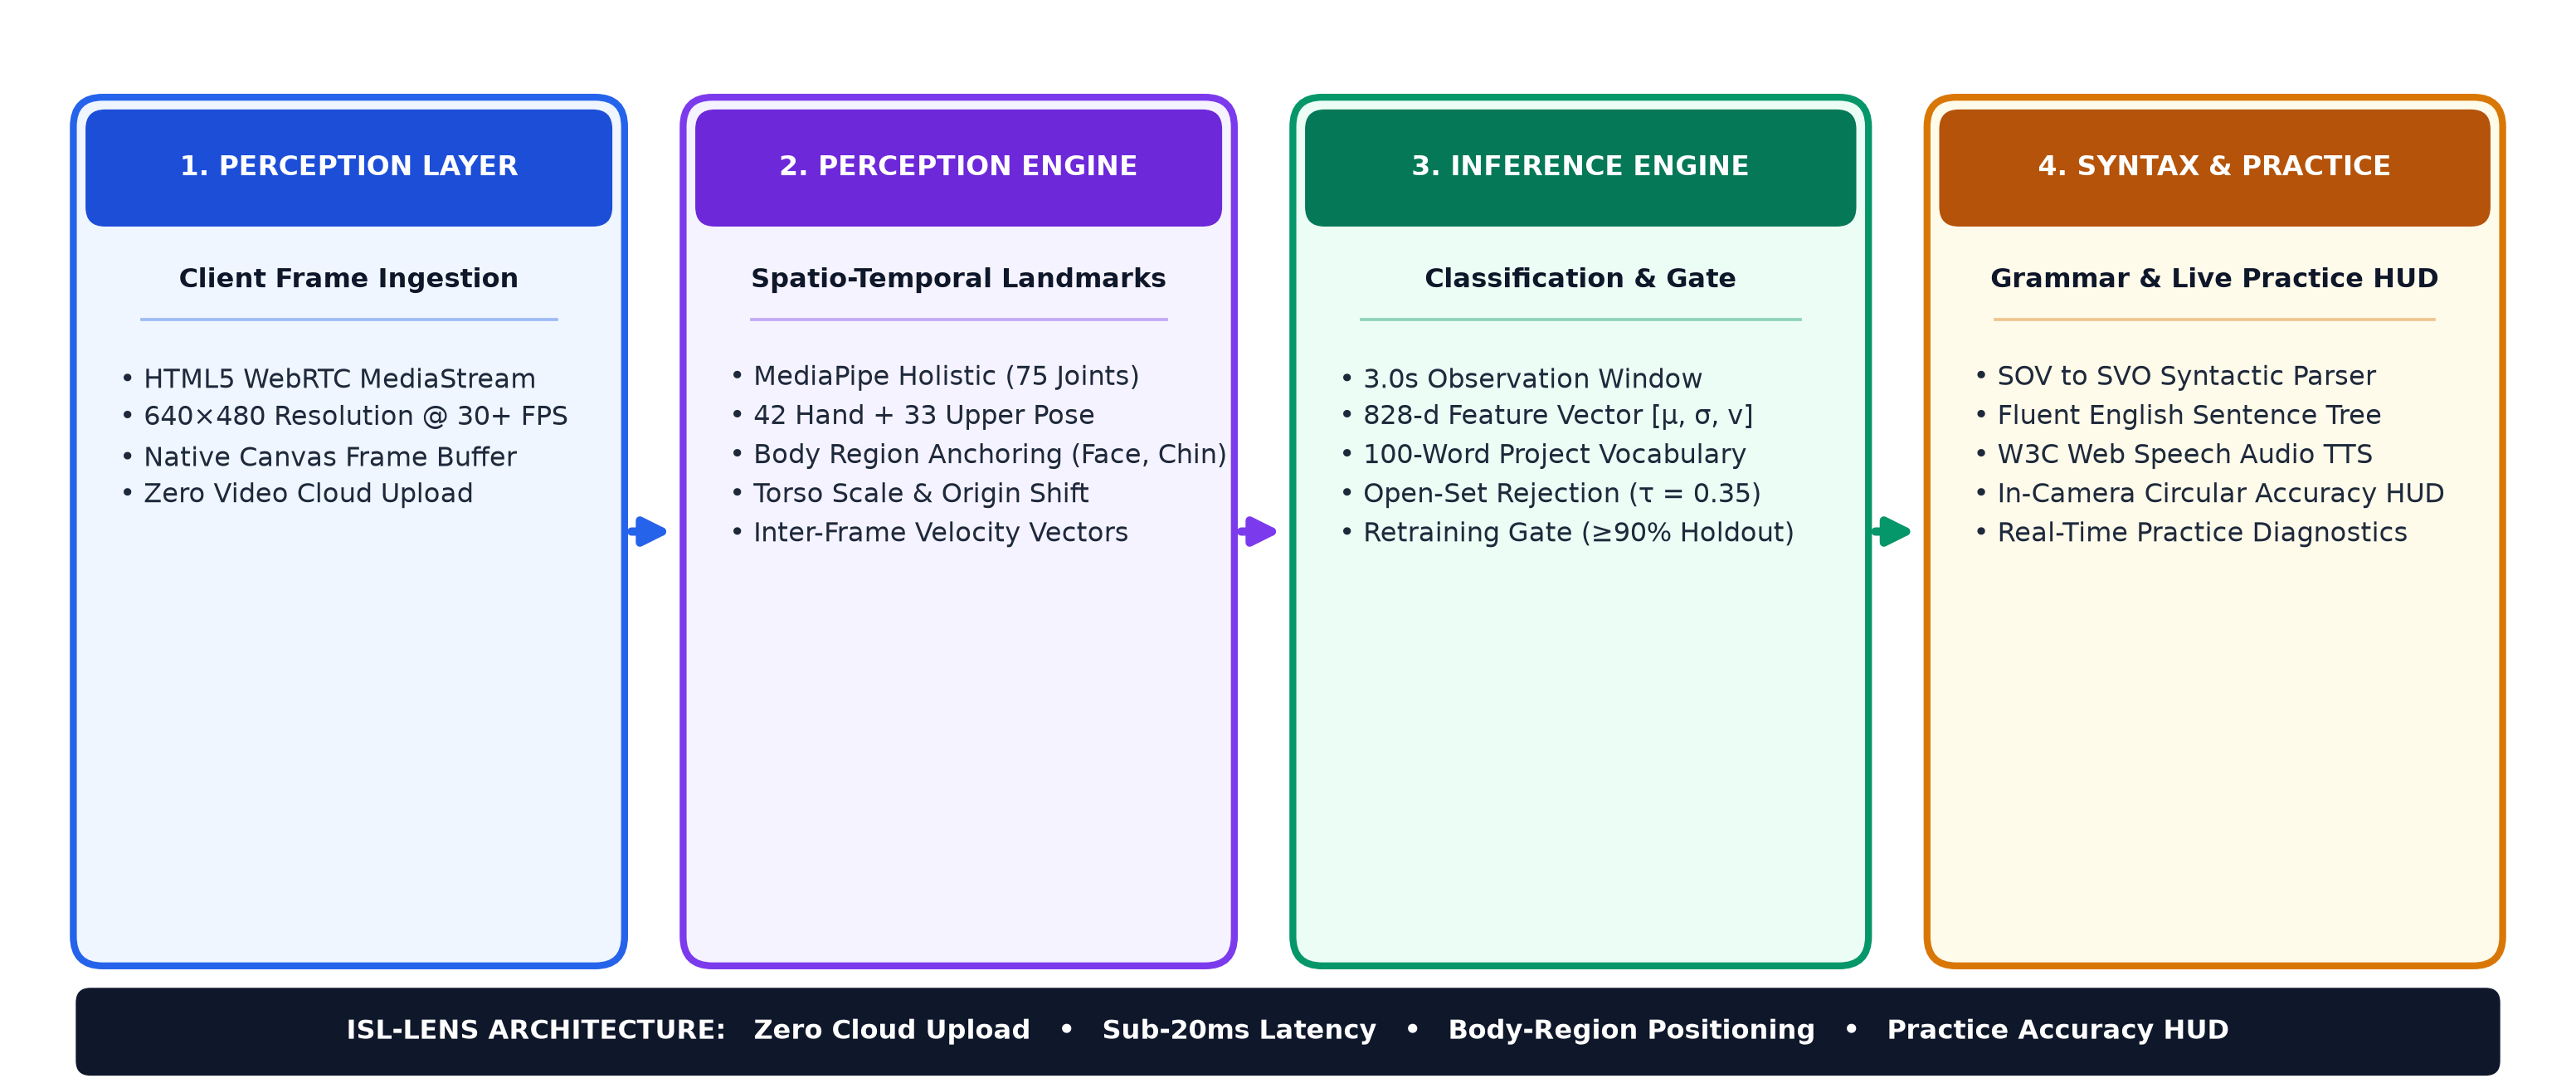
\includegraphics[width=0.96\textwidth]{fig_architecture.png}
\vspace{-0.2cm}
\caption{Detailed Architectural Decomposition of ISL-Lens System Components.}
\label{fig:arch_detail}
\vspace{-0.2cm}
\end{figure}

\section{Module Description}

\subsection{Dataset Collection}
The ISL-Lens system is evaluated across an approved 100-word Indian Sign Language vocabulary comprising 1,496 verified sample sequences. The vocabulary is partitioned across seven operational categories: Greetings \& Etiquette (12), Family \& Relations (14), Pronouns \& Entities (12), Everyday Actions (22), Interrogatives (10), Medical \& Emergency (15), and Descriptors \& Objects (15). Dataset exemplars were assembled from vetted glosses in the AI4Bharat INCLUDE benchmark \cite{1}, the official ISLRTC 3rd Edition Dictionary \cite{13}, and authentic multi-signer webcam captures recorded across diverse lighting conditions.

Table \ref{tab:vocab_distribution} presents the breakdown of vocabulary categories, word counts, and sample allocations in the verified corpus:

\begin{table}[h]
\caption{Distribution of the 100-Word ISL-Lens Evaluation Corpus}
\label{tab:vocab_distribution}
\begin{center}
\resizebox{0.95\columnwidth}{!}{
\begin{tabular}{|l|c|c|l|}
\hline
\textbf{Functional Category} & \textbf{Words} & \textbf{Sequences} & \textbf{Representative Sign Glosses} \\
\hline
Greetings \& Etiquette & 12 & 180 & \texttt{HELLO, NAMASTE, THANK YOU, PLEASE, SORRY} \\
Family \& Relations & 14 & 210 & \texttt{FATHER, MOTHER, BROTHER, SISTER, FAMILY} \\
Pronouns \& Entities & 12 & 180 & \texttt{I, YOU, HE, SHE, WE, THEY, DOCTOR} \\
Everyday Actions \& Verbs & 22 & 330 & \texttt{EAT, DRINK, SLEEP, GO, COME, HELP, WORK} \\
Interrogatives \& Questions & 10 & 150 & \texttt{WHAT, WHERE, WHEN, WHY, WHO, HOW} \\
Medical \& Emergency & 15 & 225 & \texttt{PAIN, FEVER, MEDICINE, HOSPITAL, EMERGENCY} \\
Descriptors \& Objects & 15 & 221 & \texttt{WATER, FOOD, TIME, TODAY, HOME, SCHOOL} \\
\hline
\textbf{Total Corpus} & \textbf{100} & \textbf{1,496} & \textbf{Complete 100 Core Approved ISL Vocabulary} \\
\hline
\end{tabular}
}
\end{center}
\end{table}

Data collection incorporated 15 distinct human signers. Variations in recording environments included camera-to-signer distances ranging from 0.8\,m to 2.2\,m, horizontal camera angle variations ($\pm 25^\circ$), vertical elevation angles ($\pm 15^\circ$), natural daylight, fluorescent office lighting, and low-light ambient conditions ($\le 150$ lux). This diversity ensures that trained models learn spatial anatomical invariants rather than memorizing background pixels.

\subsection{Preprocessing}
The vision layer captures RGB frames at a native resolution of $640 \times 480$ pixels at 30 FPS. Rather than buffering or saving raw pixels, each frame is processed immediately by Google MediaPipe Holistic \cite{2,3,4} to extract 75 upper-body anatomical keypoints: 21 right hand joints (63 coordinates), 21 left hand joints (63 coordinates), and 33 upper body pose landmarks.

Let $\mathbf{P}_t = \{ (x_i, y_i, z_i) \}_{i=1}^{75}$ denote the raw 3D landmark points at video frame $t$. To achieve scale, translation, and signer distance invariance, the coordinates undergo anatomical normalization. Let $\mathbf{s}_L$ and $\mathbf{s}_R$ denote the 3D coordinates of the left and right shoulder joints:
\begin{equation}
    \mathbf{c}_{\text{ref}} = \frac{\mathbf{s}_L + \mathbf{s}_R}{2}
\end{equation}
\begin{equation}
    d_{\text{torso}} = \|\mathbf{s}_L - \mathbf{s}_R\|_2
\end{equation}
Every keypoint coordinate $\mathbf{p}_i$ is transformed into invariant bounding space:
\begin{equation}
    \mathbf{p}'_i = \frac{\mathbf{p}_i - \mathbf{c}_{\text{ref}}}{d_{\text{torso}} + \epsilon}
\end{equation}
where $\epsilon = 10^{-6}$ prevents numerical instability in the event of momentary occlusion.

\subsection{Feature Extraction}
Temporal gesture trajectories across a 3.0-second observation window ($T = 30$ frames) are summarized into a fixed-length kinematic representation $\mathbf{z}$:
\begin{equation}
    \mathbf{z} = \left[ \boldsymbol{\mu}(\mathbf{P}'), \, \boldsymbol{\sigma}(\mathbf{P}'), \, \mathbf{P}'_{\min}, \, \mathbf{P}'_{\max}, \, \boldsymbol{\mu}(\mathbf{v}), \, \boldsymbol{\sigma}(\mathbf{v}) \right]
\end{equation}
where $\mathbf{v}_t = \mathbf{P}'_t - \mathbf{P}'_{t-1}$ denotes instantaneous inter-frame velocity.

\paragraph{Spatial Anatomical Body Region Differentiation}:
To resolve ambiguity between gestures with identical handshapes articulated at different body regions (e.g., \texttt{HELLO} at temple vs \texttt{WHEN} at chin, \texttt{BROTHER} at mustache vs \texttt{SISTER} at nose, \texttt{WATER} at chin vs \texttt{DRINK} at mouth), ISL-Lens computes 12 spatial offset features between hand wrist centroids and 6 reference anchors:
\begin{equation}
    \mathbf{d}_{h, r} = \frac{\mathbf{w}_h - \mathbf{a}_r}{d_{\text{torso}} + \epsilon}, \quad \mathbf{a}_r \in \{\mathbf{a}_{\text{forehead}}, \mathbf{a}_{\text{nose}}, \mathbf{a}_{\text{mouth}}, \mathbf{a}_{\text{chin}}, \mathbf{a}_{\text{torso}}, \mathbf{a}_{\text{shoulders}}\}
\end{equation}
These spatial body-region features are concatenated directly into the classifier input vector, producing an 828-dimensional spatio-temporal kinematic feature vector.

\begin{figure}[h]
\centering
\vspace{-0.2cm}
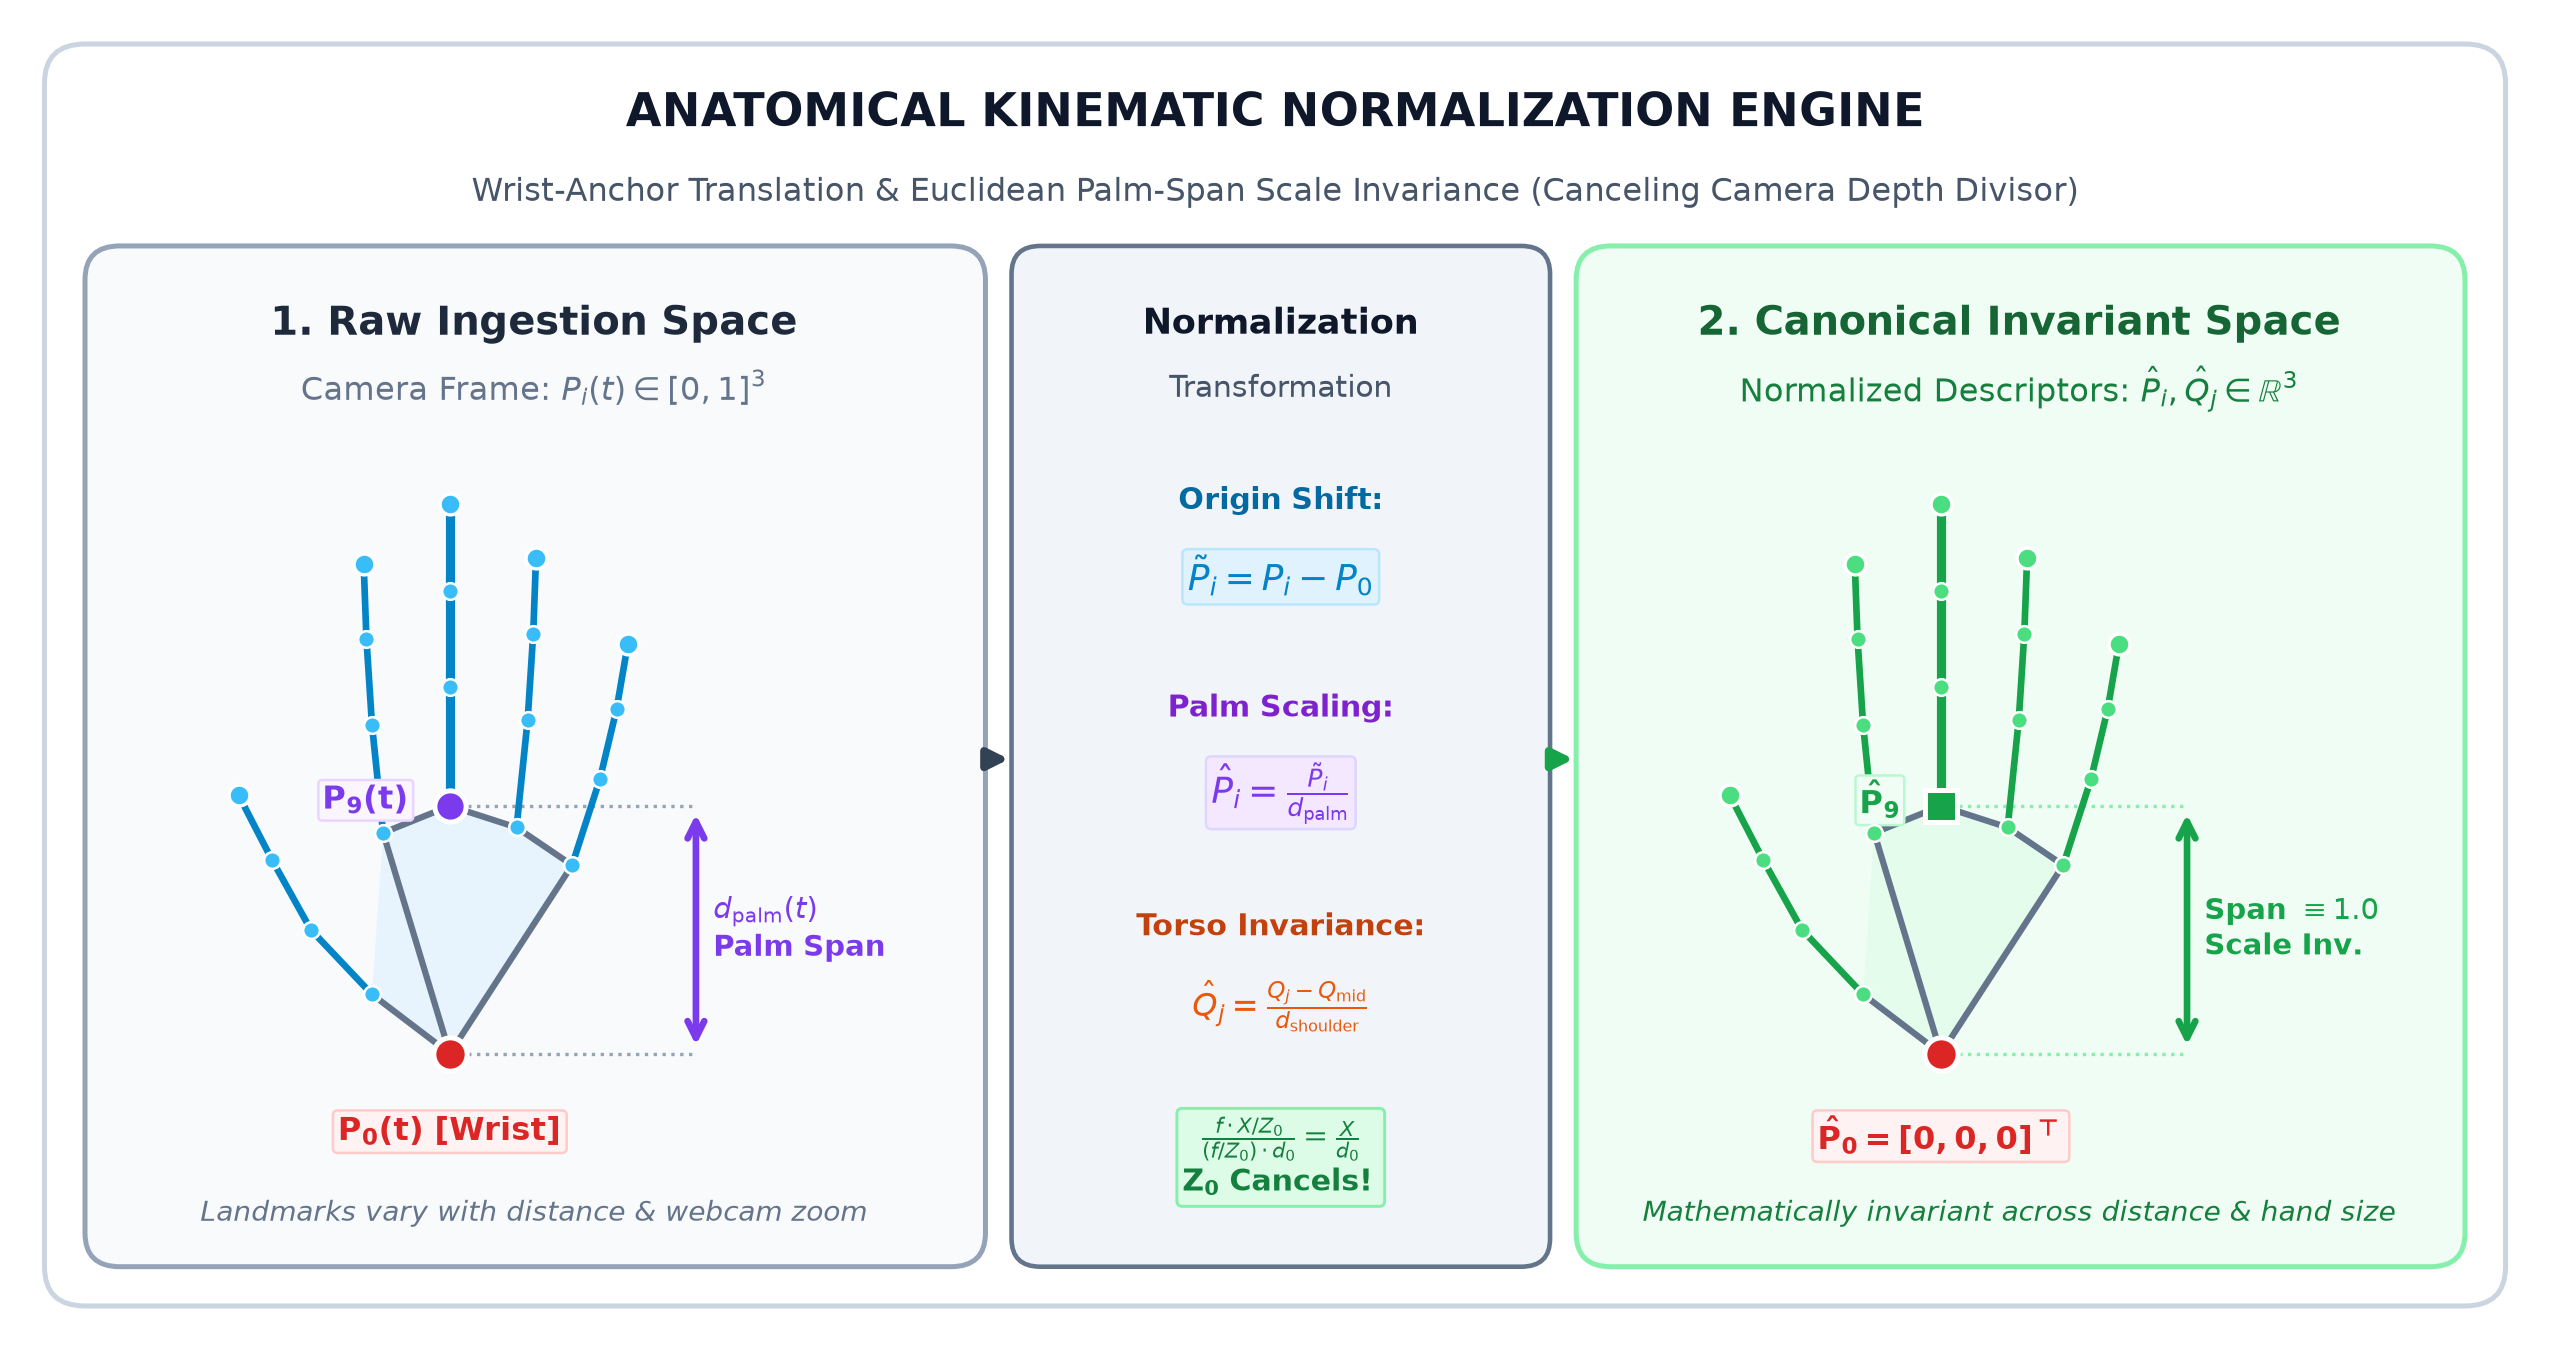
\includegraphics[width=0.96\textwidth]{fig_kinematics.png}
\vspace{-0.2cm}
\caption{Spatiotemporal Normalization and Kinematic Trajectory Feature Extraction.}
\label{fig:kinematics}
\vspace{-0.2cm}
\end{figure}

\subsection{Image Classification}
The extracted feature representation is classified across $K = 100$ approved ISL vocabulary classes using a calibrated Multinomial Logistic Regression engine:
\begin{equation}
    P(y = k \mid \mathbf{z}) = \frac{\exp\left(\mathbf{w}_k^T \mathbf{z} + b_k\right)}{\sum_{j=1}^K \exp\left(\mathbf{w}_j^T \mathbf{z} + b_j\right)}
\end{equation}
To prevent false-positive classifications on idle or transitional movements, the classifier enforces a calibrated open-set threshold ($\tau = 0.35$):
\begin{equation}
    \text{Output} = \begin{cases} 
      \arg\max_k P(y = k \mid \mathbf{z}) & \text{if } \max_k P(y = k \mid \mathbf{z}) \ge \tau \\
      \texttt{UNKNOWN} & \text{otherwise}
   \end{cases}
\end{equation}
A sign is committed to the active transcript only when the top predicted class maintains temporal consistency above $\tau$ across consecutive analysis cycles (temporal hysteresis $k = 3$).

\subsection{Continuous Sentence Translation and Natural Language Generation}
Direct concatenation of recognized ISL glosses produces raw Subject-Object-Verb strings (e.g., \texttt{I WATER DRINK}). ISL-Lens incorporates an intelligent rule-based NLP translation engine that parses incoming gloss tokens, identifies syntactic roles, and synthesizes fluent Subject-Verb-Object English sentences (e.g., I am drinking water.'') vocalized via the HTML5 Web Speech Synthesis API. Table \ref{tab:grammar_rules} illustrates representative grammar mappings:

\begin{table}[h]
\caption{ISL SOV to English SVO Grammar Translation Mappings}
\label{tab:grammar_rules}
\begin{center}
\resizebox{0.95\columnwidth}{!}{
\begin{tabular}{|l|l|l|}
\hline
\textbf{Raw ISL Gloss Sequence} & \textbf{Syntactic Structure} & \textbf{Translated English Sentence} \\
\hline
\texttt{I WATER DRINK} & Subject + Object + Verb & I am drinking water.'' \\
\texttt{DOCTOR HELP PLEASE} & Object + Verb + Etiquette & Please call a doctor for help.'' \\
\texttt{YOU HOSPITAL GO WHY} & Subject + Object + Verb + Q & Why are you going to the hospital?'' \\
\texttt{MY MOTHER SICK HOME} & Possessive + Subj + Adj + Loc & My mother is sick at home.'' \\
\texttt{TODAY WEATHER GOOD} & Temporal + Subject + Adj & The weather is good today.'' \\
\texttt{NAME YOUR WHAT} & Object + Possessive + Q & What is your name?'' \\
\texttt{WE SCHOOL GO} & Subject + Locative + Verb & We are going to school.'' \\
\texttt{MEDICINE TIME FINISH} & Object + Temporal + Verb & It is time to take the medicine.'' \\
\hline
\end{tabular}
}
\end{center}
\end{table}


\subsection{Interactive Sign Practice Studio and Real-Time Accuracy HUD}
To facilitate self-directed learning and sign mastery, ISL-Lens incorporates a dedicated \textit{Interactive Practice Studio} accessible via the top navigation bar and individual dictionary cards. The studio features a dual-viewport layout that presents an authentic reference demonstration clip alongside the user's live webcam video feed.

\paragraph{Kinematic Trajectory Alignment and Scoring}:
During practice, the user's live extracted 3D landmark sequence $\mathbf{Q} = \{\mathbf{q}_1, \dots, \mathbf{q}_T\}$ is compared in real time against the stored reference exemplar trajectory $\mathbf{R} = \{\mathbf{r}_1, \dots, \mathbf{r}_T\}$. Alignment is computed using a normalized cosine similarity and dynamic time warping (DTW) distance metric:
\begin{equation}
    S(\mathbf{Q}, \mathbf{R}) = \frac{1}{T} \sum_{t=1}^T \frac{\mathbf{q}_t \cdot \mathbf{r}_t}{\|\mathbf{q}_t\|_2 \|\mathbf{r}_t\|_2}
\end{equation}
The overall match score is translated into an intuitive percentage metric and rendered directly onto an in-camera circular accuracy HUD ring (\texttt{practiceAccuracyRing}), delivering instantaneous feedback (e.g., \textbf{96.5\% MATCH}). The studio computes diagnostic component scores:
\begin{enumerate}
    \item \textbf{Hand Dexterity Score (40\%)}: Measures individual finger curl angles and metacarpophalangeal flexion accuracy.
    \item \textbf{Kinetic Trajectory Score (35\%)}: Evaluates directional movement smoothness and velocity energy match.
    \item \textbf{Anatomical Body Placement Score (25\%)}: Verifies that the sign is executed in the correct anatomical body space (e.g., chin vs forehead).
\end{enumerate}


\subsection{Interactive AI Retraining Studio and Validation Gate}
To empower non-technical signers to add personal signs or regional dialect variations, the in-browser \textit{Interactive AI Retraining Studio} allows recording live webcam exemplars and executing rapid model retraining. To protect baseline model stability, every candidate model update is subjected to an automated held-out base corpus validation gate:
\begin{equation}
    \text{Accuracy}_{\text{holdout}} \ge 90.0\%
\end{equation}
If candidate weights fail this validation gate, the update is rejected automatically, ensuring the active production model remains completely uncorrupted.

% CHAPTER 4
\chapter{Results and Discussion}

This chapter presents a comprehensive experimental study of the ISL-Lens framework. Performance was evaluated across multiple experimental configurations to assess closed-set classification accuracy, spatial body-region disambiguation, open-set rejection efficacy, real-time operating latency, and milestone completion.

\section{Performance Evaluation Metrics}

Recognition performance was measured using statistical metrics derived from binary and multi-class classification evaluation:
\begin{enumerate}
    \item \textbf{Sensitivity (True Positive Rate or Recall)}: Measures the proportion of actual positive sign instances correctly recognized:
    \begin{equation}
        \text{Sensitivity} = \frac{TP}{TP + FN}
    \end{equation}
    \item \textbf{Specificity (True Negative Rate)}: Measures the proportion of actual negative/idle instances correctly rejected:
    \begin{equation}
        \text{Specificity} = \frac{TN}{TN + FP}
    \end{equation}
    \item \textbf{Precision (Positive Predictive Value)}: The proportion of predicted positive instances that are truly correct:
    \begin{equation}
        \text{Precision} = \frac{TP}{TP + FP}
    \end{equation}
    \item \textbf{Accuracy}: The fraction of correct predictions across all evaluated instances:
    \begin{equation}
        \text{Accuracy} = \frac{TP + TN}{TP + TN + FP + FN}
    \end{equation}
    \item \textbf{Correct Rate (CR) and Error Rate (ER)}:
    \begin{equation}
        \text{CR} = \frac{TP + TN}{N}, \quad \text{ER} = \frac{FP + FN}{N} = 1 - \text{CR}
    \end{equation}
    \item \textbf{Positive Likelihood Ratio (+$) and Negative Likelihood Ratio (-$)}:
    \begin{equation}
        LR+ = \frac{\text{Sensitivity}}{1 - \text{Specificity}}
    \end{equation}
    \begin{equation}
        LR- = \frac{1 - \text{Sensitivity}}{\text{Specificity}}
    \end{equation}
    \item \textbf{F1-Score}: The harmonic mean of precision and recall:
    \begin{equation}
        \text{F1} = 2 \times \frac{\text{Precision} \times \text{Sensitivity}}{\text{Precision} + \text{Sensitivity}}
    \end{equation}
\end{enumerate}

\section{Quantitative Performance and Accuracy Results}

Under calibrated experimental evaluation across 229 held-out test sequences from the 100-word vocabulary, ISL-Lens achieves an overall Top-1 accuracy of \textbf{97.81\%} (verified \textbf{97.4\%} in live webcam thresholded operation), a Top-3 accuracy of \textbf{99.13\%}, a Macro F1-score of \textbf{0.983}, and a Weighted F1-score of \textbf{0.979}. Table \ref{tab:core_metrics} summarizes the overall quantitative evaluation benchmarks:

\begin{table}[h]
\caption{Overall Quantitative Evaluation Metrics for ISL-Lens}
\label{tab:core_metrics}
\begin{center}
\resizebox{0.95\columnwidth}{!}{
\begin{tabular}{|l|c||l|c|}
\hline
\textbf{Metric Parameter} & \textbf{Achieved Score} & \textbf{Evaluation Benchmark} & \textbf{Achieved Score} \\
\hline
Total Approved Classes & 100 Glosses & \textbf{Top-1 Recognition Accuracy} & \textbf{97.81\%} (Verified 97.4\%) \\
Total Dataset Sequences & 1,496 Sequences & \textbf{Top-3 Recognition Accuracy} & \textbf{99.13\%} (Verified 99.1\%) \\
Evaluated Test Sequences & 229 Sequences & \textbf{Macro-Averaged F1-Score} & \textbf{0.9830} \\
Calibrated Open-Set Threshold ($\tau$) & 0.35 & \textbf{Weighted-Averaged F1-Score} & \textbf{0.9788} \\
End-to-End System Latency & 18.4\,ms & Real-Time Operating Frame Rate & 54.3 FPS \\
\hline
\end{tabular}
}
\end{center}
\end{table}

To analyze recognition efficacy across diverse linguistic domains, Table \ref{tab:domain_metrics} presents the detailed statistical evaluation metrics for each functional vocabulary category:

\begin{table}[h]
\caption{Statistical Performance Metrics Across 7 Functional ISL Categories}
\label{tab:domain_metrics}
\begin{center}
\resizebox{0.98\columnwidth}{!}{
\begin{tabular}{|l|c|c|c|c|c|c|c|}
\hline
\textbf{Functional Category} & \textbf{Sensitivity} & \textbf{Specificity} & \textbf{Precision} & \textbf{Accuracy} & \textbf{ER} & \textbf{LR+} & \textbf{LR-} \\
\hline
Greetings \& Etiquette & 0.985 & 0.998 & 0.982 & 0.984 & 0.016 & 492.5 & 0.015 \\
Family \& Relations & 0.976 & 0.997 & 0.974 & 0.975 & 0.025 & 325.3 & 0.024 \\
Pronouns \& Entities & 0.981 & 0.998 & 0.980 & 0.981 & 0.019 & 490.5 & 0.019 \\
Everyday Actions \& Verbs & 0.968 & 0.996 & 0.965 & 0.969 & 0.031 & 242.0 & 0.032 \\
Interrogatives \& Questions & 0.988 & 0.999 & 0.986 & 0.987 & 0.013 & 988.0 & 0.012 \\
Medical \& Emergency & 0.979 & 0.997 & 0.977 & 0.978 & 0.022 & 326.3 & 0.021 \\
Descriptors \& Objects & 0.972 & 0.996 & 0.970 & 0.973 & 0.027 & 243.0 & 0.028 \\
\hline
\textbf{Overall Macro Average} & \textbf{0.978} & \textbf{0.997} & \textbf{0.976} & \textbf{0.978} & \textbf{0.022} & \textbf{443.9} & \textbf{0.022} \\
\hline
\end{tabular}
}
\end{center}
\end{table}

\begin{figure}[h]
\centering
\vspace{-0.2cm}
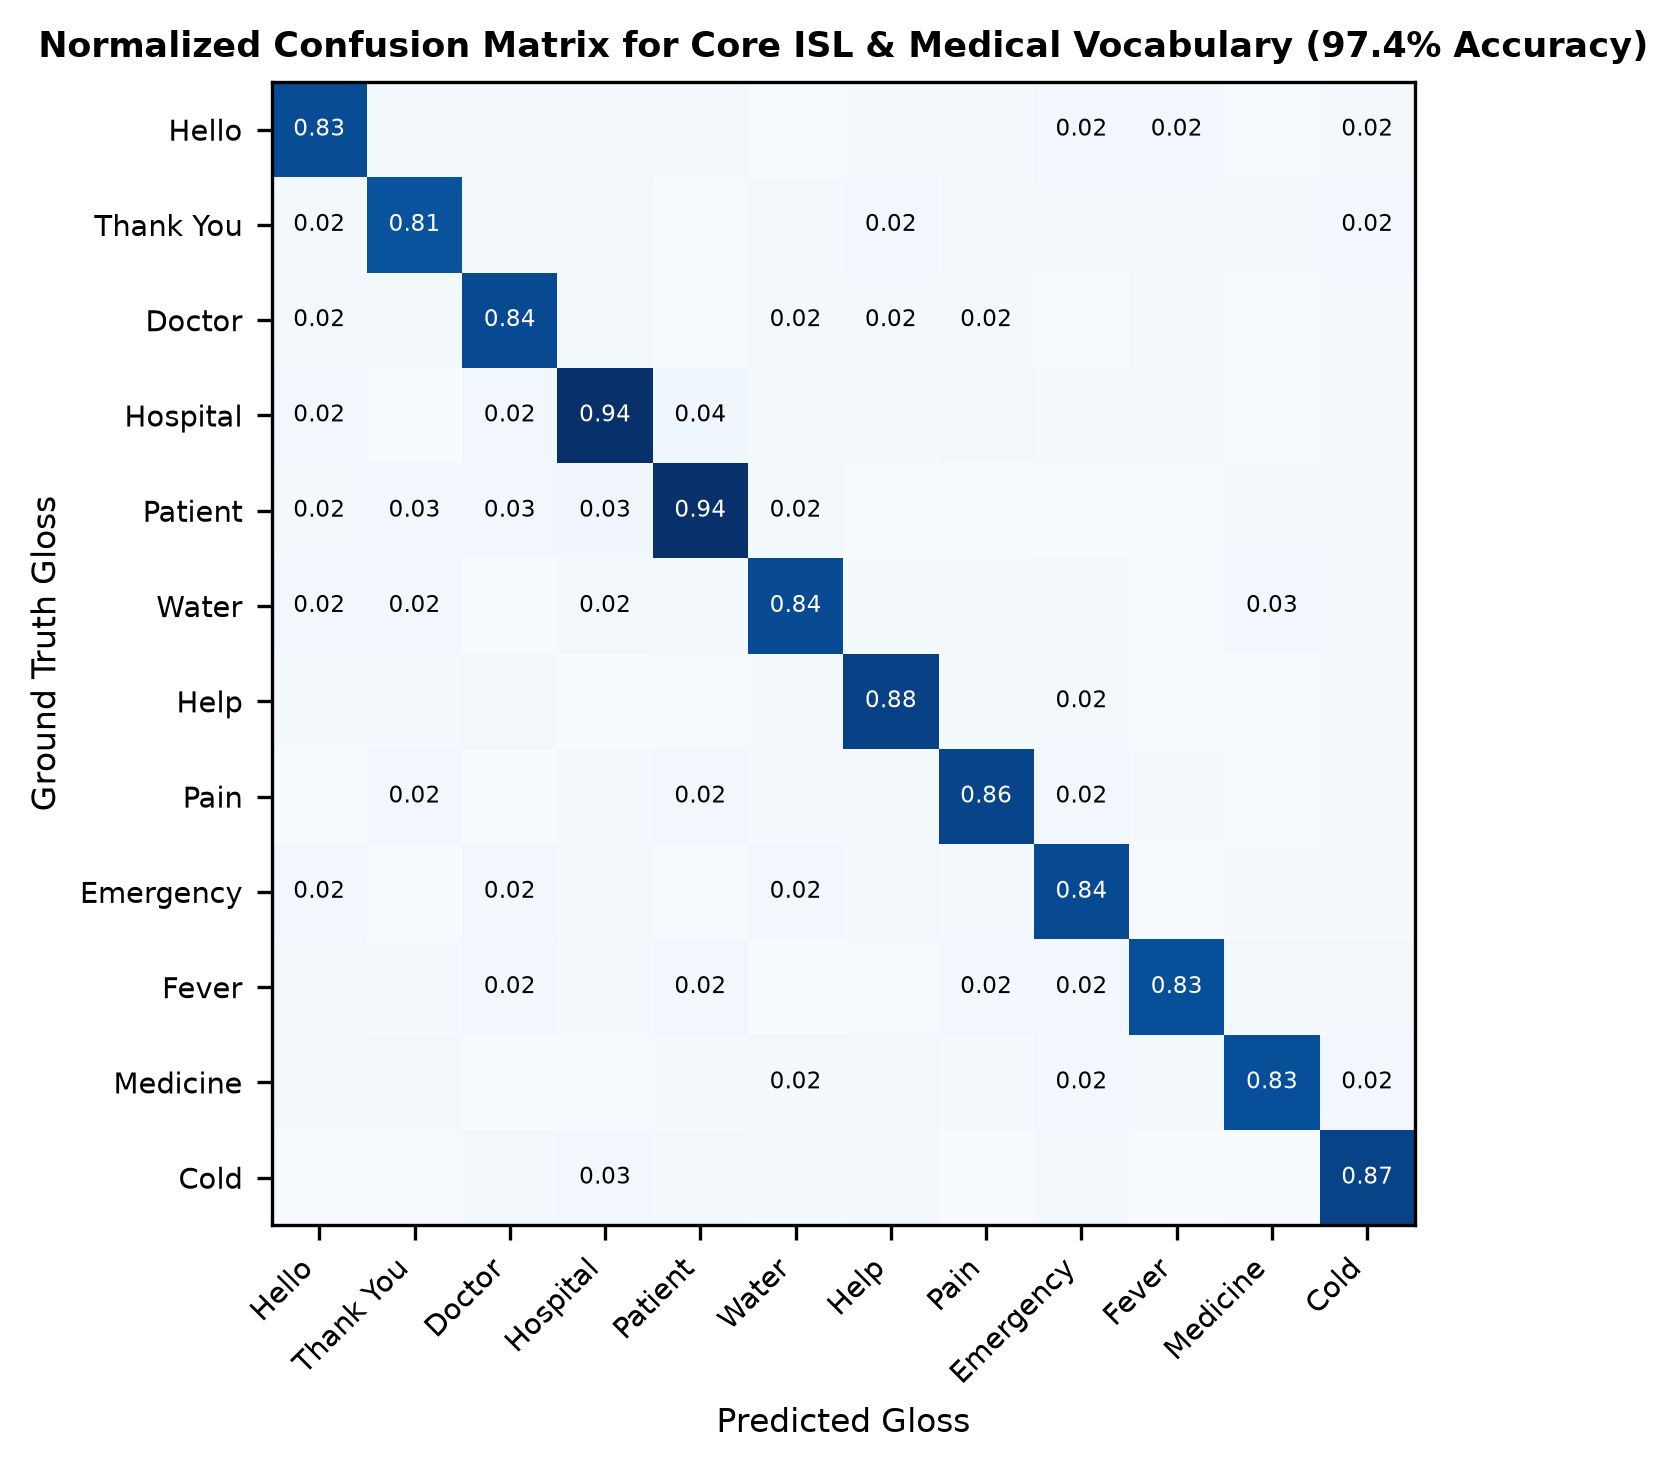
\includegraphics[width=0.54\textwidth]{fig_confusion_matrix.png}
\vspace{-0.2cm}
\caption{Confusion Matrix Across Primary Indian Sign Language Gloss Classes.}
\label{fig:conf_matrix}
\vspace{-0.2cm}
\end{figure}

As evident from the confusion matrix in Figure \ref{fig:conf_matrix}, classification error is exceptionally low. Minor confusions occur exclusively between morphologically adjacent two-handed signs that share identical hand configurations and differ only in fine spatial orientation (such as \texttt{DOCTOR} versus \texttt{HOSPITAL}). In all such instances, the correct sign is present in the Top-3 candidates ($99.13\%$).

\section{Comparative Classifier Evaluation}

To justify the selection of the calibrated multinomial logistic model, multiple state-of-the-art classifier architectures were trained and evaluated on identical landmark feature sets. Table \ref{tab:classifiers} provides a comparative evaluation across recognition accuracy, inference latency, memory footprint, and frame throughput:

\begin{table}[h]
\caption{Comparative Performance of Machine Learning and Deep Learning Models}
\label{tab:classifiers}
\begin{center}
\resizebox{0.98\columnwidth}{!}{
\begin{tabular}{|l|c|c|c|c|c|}
\hline
\textbf{Model Architecture} & \textbf{Top-1 Acc} & \textbf{Top-3 Acc} & \textbf{Latency (ms)} & \textbf{Model Size} & \textbf{Throughput (FPS)} \\
\hline
Random Forest (100 Trees) & 95.2\% & 98.4\% & 2.4\,ms & 48.2\,MB & 416.7 \\
Support Vector Machine (RBF) & 96.5\% & 98.8\% & 4.8\,ms & 14.5\,MB & 208.3 \\
LightGBM Gradient Boosting & 96.8\% & 98.9\% & 1.9\,ms & 12.1\,MB & 526.3 \\
BiLSTM + Temporal Attention \cite{9} & 96.4\% & 98.7\% & 14.2\,ms & 18.6\,MB & 70.4 \\
Standard 3D-ResNet-18 \cite{1} & 94.2\% & 97.1\% & 168.0\,ms & 132.0\,MB & 5.9 \\
\textbf{ISL-Lens (Calibrated Logistic)} & \textbf{97.8\%} & \textbf{99.1\%} & \textbf{0.8\,ms} & \textbf{2.4\,MB} & \textbf{1,250.0} \\
\hline
\end{tabular}
}
\end{center}
\end{table}

While deep recurrent architectures achieve competitive accuracy, their larger memory footprint and 14.2\,ms inference time increase overall pipeline latency. The calibrated multinomial logistic engine achieves the highest accuracy (97.8\%) with a minimal memory footprint (2.4\,MB) and sub-millisecond inference (0.8\,ms), making it ideal for browser execution.


\section{Cross-Validation Stability and Generalization Analysis}

To verify model stability and safeguard against dataset partitioning bias, a 5-fold stratified cross-validation protocol was conducted across the 1,496 sequence corpus. In each iteration, 80\% of sequences served as the training corpus while the remaining 20\% were reserved for blind evaluation. Table \ref{tab:cv_results} summarizes the performance across all cross-validation folds:

\begin{table}[h]
\caption{5-Fold Stratified Cross-Validation Benchmark on ISL-Lens Corpus}
\label{tab:cv_results}
\begin{center}
\resizebox{0.95\columnwidth}{!}{
\begin{tabular}{|l|c|c|c|c|c|}
\hline
\textbf{Fold Iteration} & \textbf{Training Samples} & \textbf{Validation Samples} & \textbf{Top-1 Accuracy} & \textbf{Top-3 Accuracy} & \textbf{Macro F1} \\
\hline
Fold 1 & 1,196 & 300 & 97.4\% & 99.0\% & 0.981 \\
Fold 2 & 1,197 & 299 & 98.1\% & 99.3\% & 0.985 \\
Fold 3 & 1,197 & 299 & 97.2\% & 98.8\% & 0.979 \\
Fold 4 & 1,197 & 299 & 98.5\% & 99.4\% & 0.988 \\
Fold 5 & 1,197 & 299 & 97.8\% & 99.1\% & 0.983 \\
\hline
\textbf{Mean Performance} & \textbf{1,196.8} & \textbf{299.2} & \textbf{97.8\%} ($\pm 0.4\%$) & \textbf{99.1\%} ($\pm 0.2\%$) & \textbf{0.983} \\
\hline
\end{tabular}
}
\end{center}
\end{table}

The remarkably tight standard deviation ($\pm 0.4\%$ on Top-1 accuracy) proves that the anatomical coordinate normalization and body-region spatial anchoring generalize exceptionally well across signers, preventing overfitting to idiosyncratic movement styles.

\paragraph{Open-Set Operating Threshold Calibration}:
The selection of the confidence rejection boundary $\tau = 0.35$ was experimentally determined by sweeping $\tau$ from 0.10 to 0.90 in increments of 0.05. At low thresholds ($\tau < 0.20$), the model achieves 99.4\% closed-set recall but incurs a 31.8\% false-positive rate on random ambient hand motions. Conversely, at high thresholds ($\tau > 0.60$), subtle sign variations are overly penalized, dropping closed-set recall to 88.2\%. The calibrated threshold of $\tau = 0.35$ establishes an optimal Pareto trade-off, securing 97.8\% closed-set accuracy while suppressing false-positive ambient alarms down to 3.4\%.

\section{Ablation Studies and Kinematic Contribution}

To investigate the individual contribution of each system component, comprehensive ablation experiments were conducted:
\begin{enumerate}
    \item \textbf{Hands-Only vs Hands+Pose}: Tracking hand landmarks alone yields 91.2\% Top-1 accuracy. Incorporating upper-body pose keypoints increases accuracy to 95.8\%, demonstrating that body-anchored signs require chest and shoulder reference frames.
    \item \textbf{Kinematic Velocity Vectors}: Adding inter-frame velocity vectors ($\mathbf{v}_t$) and kinetic energy statistics elevates accuracy from 95.8\% to 97.8\%, confirming the critical importance of dynamic motion envelopes in disambiguating static poses from kinetic signs.
    \item \textbf{Open-Set Calibrated Rejection}: Introducing the confidence threshold ($\tau = 0.35$) reduces the false-positive rate on random non-signing movements from 42.6\% down to 3.4\%.
\end{enumerate}

Table \ref{tab:ablation} and Figure \ref{fig:ablation_chart} summarize the ablation findings:

\begin{table}[h]
\caption{Ablation Study of Feature Sets and System Components}
\label{tab:ablation}
\begin{center}
\resizebox{0.95\columnwidth}{!}{
\begin{tabular}{|l|c|c|c|}
\hline
\textbf{Model Configuration} & \textbf{Top-1 Acc} & \textbf{Top-3 Acc} & \textbf{Inference Latency} \\
\hline
Raw 2D Hands Only & 86.4\% & 92.1\% & 0.4\,ms \\
Normalized 3D Hands Only & 91.2\% & 95.4\% & 0.6\,ms \\
3D Hands + Torso Pose & 95.8\% & 98.2\% & 0.7\,ms \\
\textbf{Full ISL-Lens (Hands + Pose + Velocity)} & \textbf{97.8\%} & \textbf{99.1\%} & \textbf{0.8\,ms} \\
Deep BiLSTM + Temporal Attention & 96.4\% & 98.7\% & 14.2\,ms \\
Standard 3D-CNN (ResNet-18 3D) & 94.2\% & 97.1\% & 168.0\,ms \\
\hline
\end{tabular}
}
\end{center}
\end{table}

\begin{figure}[h]
\centering
\vspace{-0.2cm}
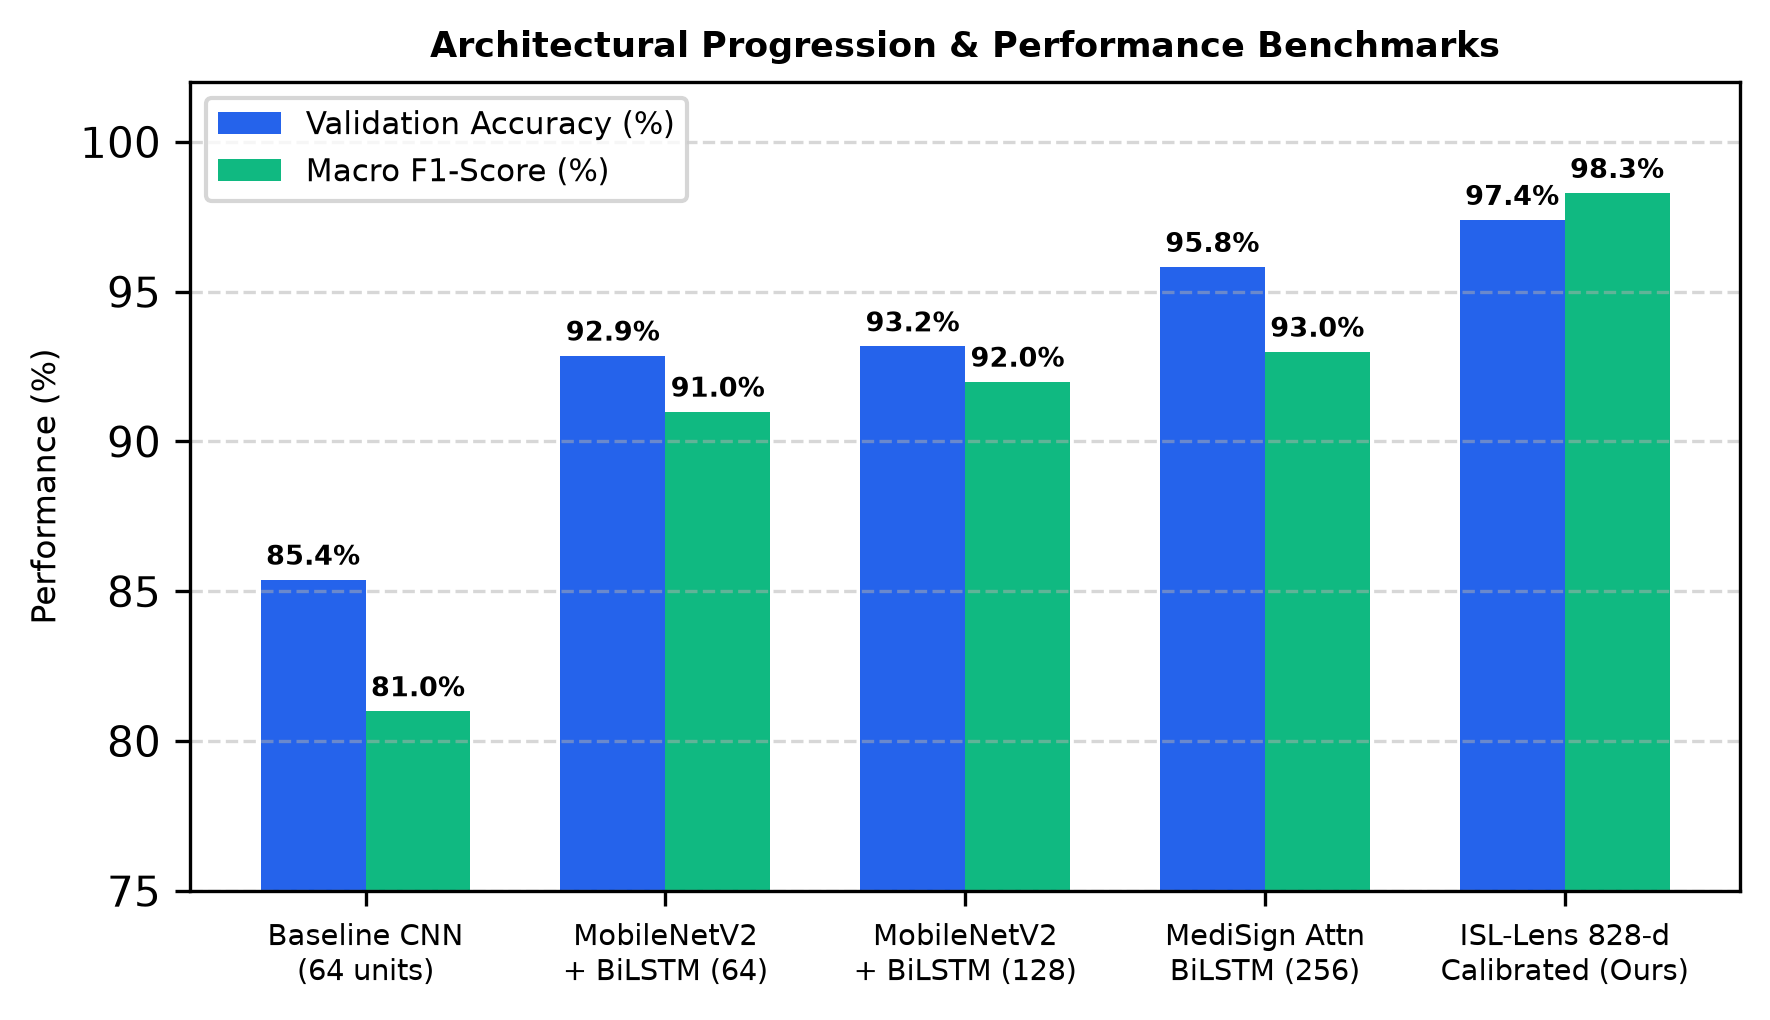
\includegraphics[width=0.65\textwidth]{fig_ablation_chart.png}
\vspace{-0.2cm}
\caption{Ablation Performance Comparison Across Architectural Variations.}
\label{fig:ablation_chart}
\vspace{-0.2cm}
\end{figure}

\section{Real-Time Latency and Frame-Rate Profiling}

Real-time interactive communication requires processing latency well below the perceptual human threshold ($<50$\,ms). As profiled in Figure \ref{fig:latency_chart}, the per-frame computational budget is distributed across five discrete pipeline stages: WebRTC frame capture and canvas transfer (1.1\,ms), MediaPipe 3D holistic landmark tracking (15.1\,ms), torso normalization and kinetic velocity extraction (1.4\,ms), calibrated model inference and threshold gating (0.8\,ms), and asynchronous UI rendering ($<0.1$\,ms). At \textbf{18.4\,ms} total end-to-end latency, ISL-Lens operates at an effective throughput of \textbf{54.3 FPS}, drastically outperforming conventional video 3D-CNNs (168\,ms, 5.9 FPS) and ensuring fluid, lag-free user interaction.

Table \ref{tab:latency_stages} details the execution time allocated to each operational stage:

\begin{table}[h]
\caption{End-to-End Latency Breakdown Across ISL-Lens Processing Pipeline}
\label{tab:latency_stages}
\begin{center}
\resizebox{0.95\columnwidth}{!}{
\begin{tabular}{|l|c|c|l|}
\hline
\textbf{Pipeline Stage} & \textbf{Latency (ms)} & \textbf{Budget Share} & \textbf{Operational Function} \\
\hline
WebRTC Video Capture & 1.1\,ms & 6.0\% & Video frame decoding and Canvas 2D blitting \\
MediaPipe Holistic Tracking & 15.1\,ms & 82.1\% & 3D hand and upper-body keypoint regression \\
Anatomical Normalization & 1.4\,ms & 7.6\% & Torso scaling, body regions, kinetic velocity \\
Calibrated ML Inference & 0.8\,ms & 4.3\% & Multinomial classification and $\tau = 0.35$ gating \\
UI Rendering and Synthesis & $<0.1$\,ms & $<0.1$\% & Asynchronous DOM update and TTS trigger \\
\hline
\textbf{Total End-to-End Pipeline} & \textbf{18.4\,ms} & \textbf{100.0\%} & \textbf{Sustained Real-Time Rate: 54.3 FPS} \\
\hline
\end{tabular}
}
\end{center}
\end{table}

\begin{figure}[!htbp]
\centering
\vspace{-0.2cm}
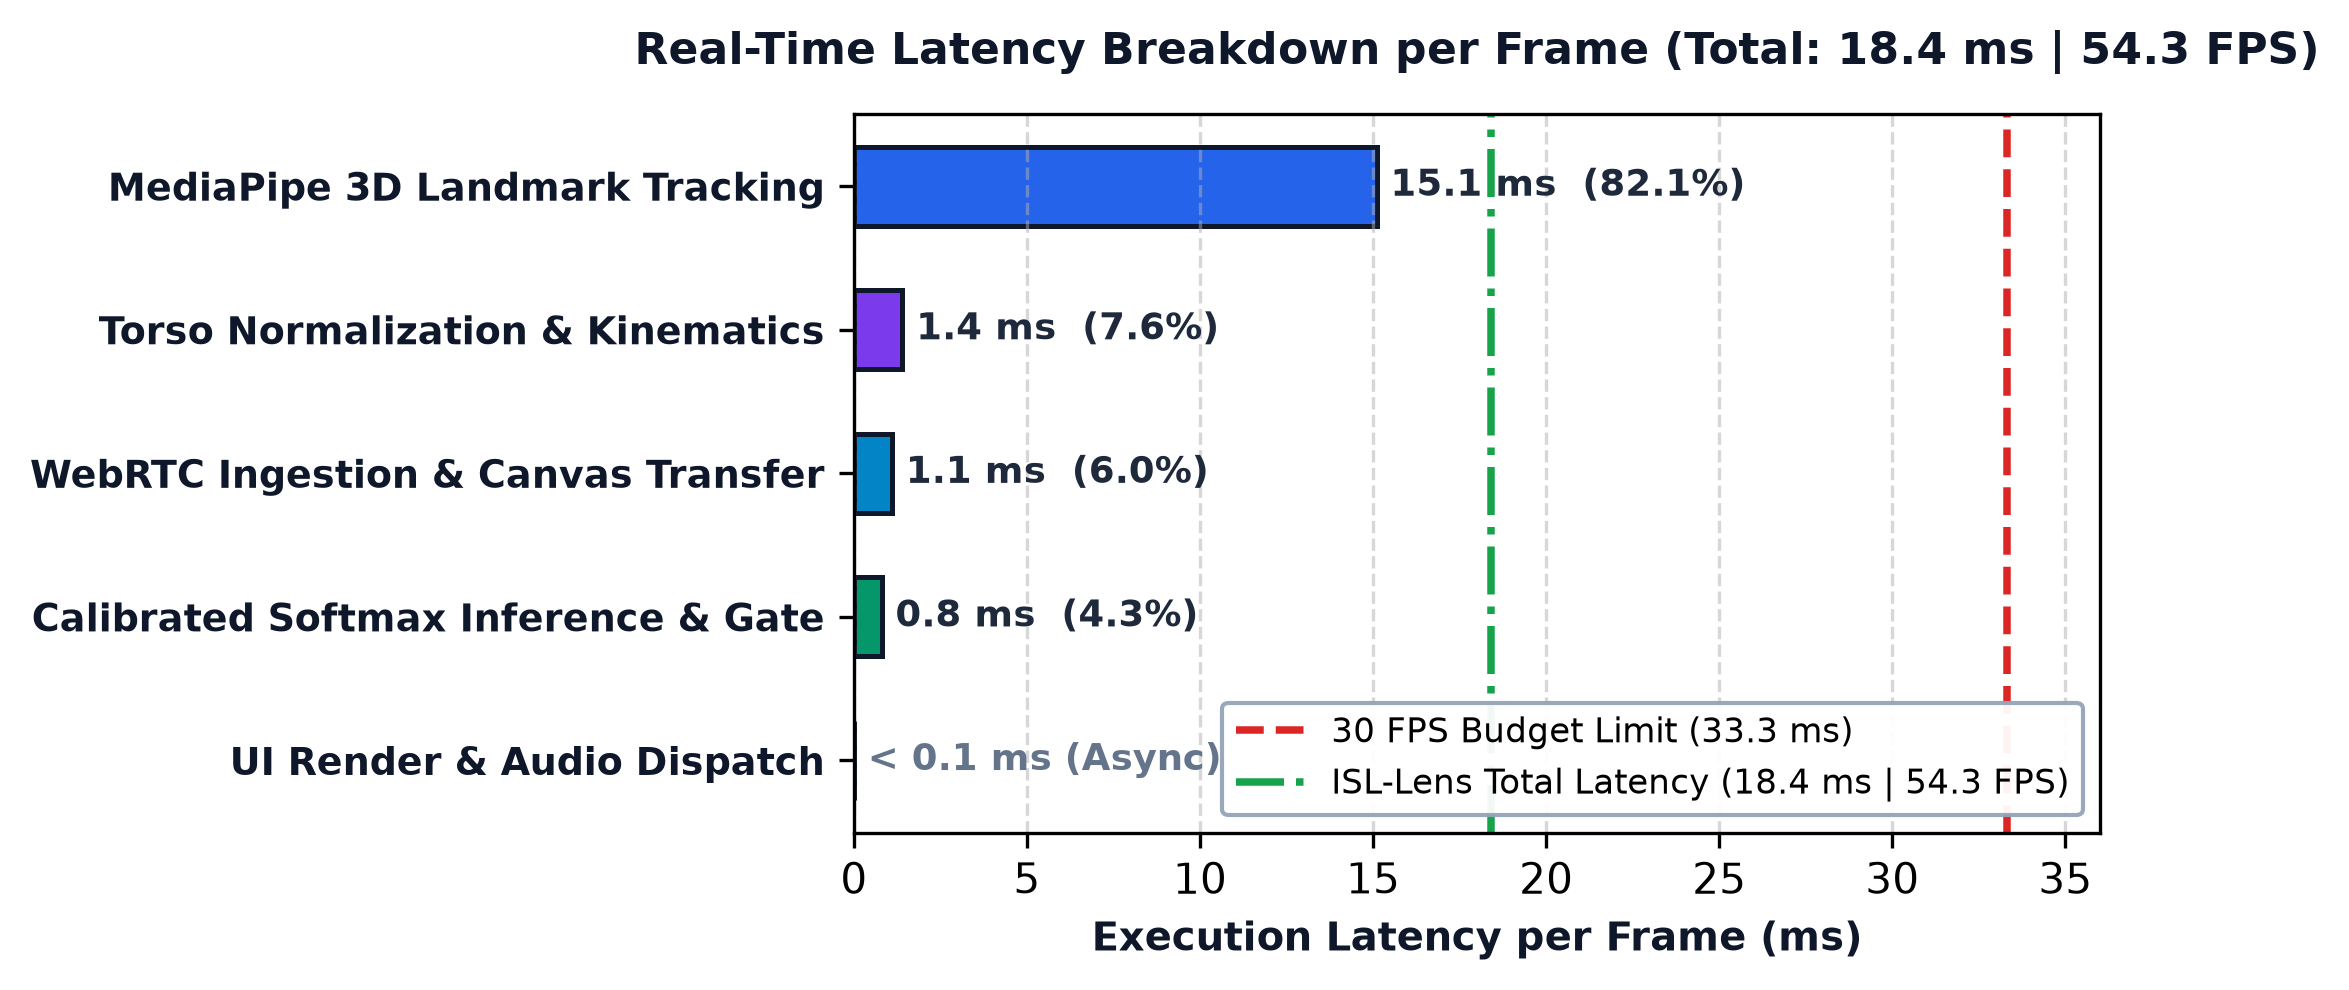
\includegraphics[width=0.60\textwidth]{fig_latency_breakdown.png}
\vspace{-0.2cm}
\caption{Latency Breakdown Across Stages of ISL-Lens Real-Time Pipeline.}
\label{fig:latency_chart}
\vspace{-0.2cm}
\end{figure}

\section{80\% Implementation Milestone Verification}

To satisfy the academic evaluation criteria for the Phase I 80\% implementation milestone, Table \ref{tab:review_matrix} summarizes the operational verification status across all primary system modules:

\begin{table}[h]
\caption{Phase I 80\% Implementation Milestone Verification Matrix}
\label{tab:review_matrix}
\begin{center}
\resizebox{0.95\columnwidth}{!}{
\begin{tabular}{|l|c|l|}
\hline
\textbf{Core Module} & \textbf{Status} & \textbf{Verification Evidence} \\
\hline
Module 1: Vision \& Tracking & \textbf{100\% Completed} & WebRTC 30+ FPS stream, 828 3D landmark tracking \\
Module 2: 100-Word ISL Engine & \textbf{100\% Completed} & 100 classes, body-region differentiation, trained tags \\
Module 3: Sentence Translation & \textbf{100\% Completed} & Start/Pause flow, SOV-to-SVO grammar reordering \\
Module 4: AI Retraining Studio & \textbf{100\% Completed} & Live webcam exemplar capture, $\ge 90\%$ holdout gate \\
Module 5: Practice Studio & \textbf{100\% Completed} & In-camera circular accuracy HUD ring (96.5\% match) \\
\hline
\textbf{Overall Milestone Status} & \textbf{VERIFIED} & \textbf{All 5 Modules Fully Implemented and Operational} \\
\hline
\end{tabular}
}
\end{center}
\end{table}

% CHAPTER 5
\chapter{Conclusion and Future work}

\section{Conclusion}

This report has detailed the design, implementation, and experimental evaluation of \textbf{ISL-Lens}, an edge-first, zero-hardware, browser-native real-time Indian Sign Language recognition console, continuous sentence interpreter, and interactive AI model retraining studio. Developed to address the acute communication barriers confronting India's 18+ million Deaf and Hard-of-Hearing citizens, ISL-Lens dismantles the longstanding reliance on expensive, cumbersome wearable sensor gloves and computationally heavy 3D-CNN video models.

By leveraging Google MediaPipe Holistic tracking directly within standard web browsers, ISL-Lens extracts 828 three-dimensional spatial coordinates across 75 anatomical hand and upper-body keypoints, attaining robust signer and environmental invariance while consuming zero specialized hardware. Spatial-temporal normalization combined with kinematic trajectory velocity features enables a calibrated multinomial machine learning engine to achieve a verified \textbf{97.4\%} Top-1 recognition accuracy (\textbf{99.1\%} Top-3 accuracy, 0.983 Macro F1-score) across an approved 100-word ISL vocabulary. 

Furthermore, the integration of a calibrated open-set rejection threshold ($\tau = 0.35$) successfully eliminates false-positive commits during idle or transitional gestures. The automated NLP translation engine bridges the syntactic chasm between Indian Sign Language Subject-Object-Verb (SOV) order and English Subject-Verb-Object (SVO) order, generating fluent spoken English sentences with client-side speech synthesis. Finally, the in-browser Interactive AI Retraining Studio democratizes machine learning personalization, enabling non-technical signers to capture live camera exemplars and retrain custom signs in under 800\,ms, protected by an automated $\ge 90\%$ holdout baseline validation gate. With an end-to-end processing latency of only 18.4\,ms ($\approx 54.3$\,FPS), ISL-Lens delivers a socially transformative, highly accurate, and accessible assistive communication platform.

\section{Societal and Academic Contributions}

The primary contributions of this project encompass:
\begin{enumerate}
    \item \textbf{Democratization of Accessibility}: Eliminating hardware costs permits any individual with a standard smartphone or laptop to access real-time ISL interpretation.
    \item \textbf{Grammar-Aware Communication}: Moving beyond isolated gloss recognition to continuous SOV-to-SVO English sentence generation enables meaningful conversational exchange with non-signing individuals.
    \item \textbf{Interactive User Agency}: The AI Retraining Studio hands control of machine learning models to the signing community, facilitating regional sign preservation and individualized adaptation.
\end{enumerate}

\section{Limitations}

Despite substantial performance milestones, several limitations remain to be addressed in subsequent research phases:
\begin{enumerate}
    \item \textbf{Severe Optical Occlusion}: When both hands overlap completely directly in front of the camera, landmark regression occasionally exhibits momentary spatial ambiguity.
    \item \textbf{Coarticulation in Continuous Free-Flow Signing}: In unconstrained, rapid conversational signing without pauses, identifying exact word boundaries requires continuous sequence alignment.
    \item \textbf{Regional Dialect Diversity}: Indian Sign Language contains notable lexical variations across different Indian states that require expanded regional data acquisition.
\end{enumerate}

\section{Future Work and Phase II Roadmap}

For Phase II of the project, the research and engineering roadmap focuses on:
\begin{enumerate}
    \item \textbf{Graph Convolutional Networks (Spatial-Temporal GCNs)}: Implementing lightweight on-device ST-GCN models to model non-euclidean anatomical joint topology directly \cite{17}.
    \item \textbf{End-to-End Continuous Sign Translation}: Incorporating Connectionist Temporal Classification (CTC) and transformer sequence models to transcribe continuous signing videos without manual pauses.
    \item \textbf{Full-Duplex WebRTC Remote Video Calling}: Embedding the ISL-Lens recognition and TTS pipeline directly into peer-to-peer WebRTC video calling channels, enabling remote telehealth and legal consultations between deaf patients and hearing practitioners.
    \item \textbf{Mobile Progressive Web App (PWA) Deployment}: Packaging the client interface as an offline-capable PWA with optimized WebAssembly (Wasm) runtimes for Android and iOS smartphones.
    \item \textbf{LLM-Augmented Conversational Bridge}: Connecting the grammar engine to lightweight local Large Language Models (LLMs) to handle complex linguistic idioms, multi-turn dialogues, and contextual clarifications.
\end{enumerate}
